\documentclass[twoside]{book}

% Packages required by doxygen
\usepackage{fixltx2e}
\usepackage{calc}
\usepackage{doxygen}
\usepackage[export]{adjustbox} % also loads graphicx
\usepackage{graphicx}
\usepackage[utf8]{inputenc}
\usepackage{makeidx}
\usepackage{multicol}
\usepackage{multirow}
\PassOptionsToPackage{warn}{textcomp}
\usepackage{textcomp}
\usepackage[nointegrals]{wasysym}
\usepackage[table]{xcolor}

% Font selection
\usepackage[T1]{fontenc}
\usepackage[scaled=.90]{helvet}
\usepackage{courier}
\usepackage{amssymb}
\usepackage{sectsty}
\renewcommand{\familydefault}{\sfdefault}
\allsectionsfont{%
  \fontseries{bc}\selectfont%
  \color{darkgray}%
}
\renewcommand{\DoxyLabelFont}{%
  \fontseries{bc}\selectfont%
  \color{darkgray}%
}
\newcommand{\+}{\discretionary{\mbox{\scriptsize$\hookleftarrow$}}{}{}}

% Page & text layout
\usepackage{geometry}
\geometry{%
  a4paper,%
  top=2.5cm,%
  bottom=2.5cm,%
  left=2.5cm,%
  right=2.5cm%
}
\tolerance=750
\hfuzz=15pt
\hbadness=750
\setlength{\emergencystretch}{15pt}
\setlength{\parindent}{0cm}
\setlength{\parskip}{3ex plus 2ex minus 2ex}
\makeatletter
\renewcommand{\paragraph}{%
  \@startsection{paragraph}{4}{0ex}{-1.0ex}{1.0ex}{%
    \normalfont\normalsize\bfseries\SS@parafont%
  }%
}
\renewcommand{\subparagraph}{%
  \@startsection{subparagraph}{5}{0ex}{-1.0ex}{1.0ex}{%
    \normalfont\normalsize\bfseries\SS@subparafont%
  }%
}
\makeatother

% Headers & footers
\usepackage{fancyhdr}
\pagestyle{fancyplain}
\fancyhead[LE]{\fancyplain{}{\bfseries\thepage}}
\fancyhead[CE]{\fancyplain{}{}}
\fancyhead[RE]{\fancyplain{}{\bfseries\leftmark}}
\fancyhead[LO]{\fancyplain{}{\bfseries\rightmark}}
\fancyhead[CO]{\fancyplain{}{}}
\fancyhead[RO]{\fancyplain{}{\bfseries\thepage}}
\fancyfoot[LE]{\fancyplain{}{}}
\fancyfoot[CE]{\fancyplain{}{}}
\fancyfoot[RE]{\fancyplain{}{\bfseries\scriptsize Generated by Doxygen }}
\fancyfoot[LO]{\fancyplain{}{\bfseries\scriptsize Generated by Doxygen }}
\fancyfoot[CO]{\fancyplain{}{}}
\fancyfoot[RO]{\fancyplain{}{}}
\renewcommand{\footrulewidth}{0.4pt}
\renewcommand{\chaptermark}[1]{%
  \markboth{#1}{}%
}
\renewcommand{\sectionmark}[1]{%
  \markright{\thesection\ #1}%
}

% Indices & bibliography
\usepackage{natbib}
\usepackage[titles]{tocloft}
\setcounter{tocdepth}{3}
\setcounter{secnumdepth}{5}
\makeindex

% Hyperlinks (required, but should be loaded last)
\usepackage{ifpdf}
\ifpdf
  \usepackage[pdftex,pagebackref=true]{hyperref}
\else
  \usepackage[ps2pdf,pagebackref=true]{hyperref}
\fi
\hypersetup{%
  colorlinks=true,%
  linkcolor=blue,%
  citecolor=blue,%
  unicode%
}

% Custom commands
\newcommand{\clearemptydoublepage}{%
  \newpage{\pagestyle{empty}\cleardoublepage}%
}

\usepackage{caption}
\captionsetup{labelsep=space,justification=centering,font={bf},singlelinecheck=off,skip=4pt,position=top}

%===== C O N T E N T S =====

\begin{document}

% Titlepage & ToC
\hypersetup{pageanchor=false,
             bookmarksnumbered=true,
             pdfencoding=unicode
            }
\pagenumbering{alph}
\begin{titlepage}
\vspace*{7cm}
\begin{center}%
{\Large Guillermo Hernández González Max Mean }\\
\vspace*{1cm}
{\large Generated by Doxygen 1.8.13}\\
\end{center}
\end{titlepage}
\clearemptydoublepage
\pagenumbering{roman}
\tableofcontents
\clearemptydoublepage
\pagenumbering{arabic}
\hypersetup{pageanchor=true}

%--- Begin generated contents ---
\chapter{Hierarchical Index}
\section{Class Hierarchy}
This inheritance list is sorted roughly, but not completely, alphabetically\+:\begin{DoxyCompactList}
\item \contentsline{section}{Algorithm}{\pageref{classAlgorithm}}{}
\begin{DoxyCompactList}
\item \contentsline{section}{Grasp}{\pageref{classGrasp}}{}
\item \contentsline{section}{greedy\+Algorithm}{\pageref{classgreedyAlgorithm}}{}
\item \contentsline{section}{Multi\+Start}{\pageref{classMultiStart}}{}
\item \contentsline{section}{second\+Greedy\+Algorithm}{\pageref{classsecondGreedyAlgorithm}}{}
\item \contentsline{section}{Vns}{\pageref{classVns}}{}
\end{DoxyCompactList}
\item \contentsline{section}{Matriz}{\pageref{classMatriz}}{}
\end{DoxyCompactList}

\chapter{Class Index}
\section{Class List}
Here are the classes, structs, unions and interfaces with brief descriptions\+:\begin{DoxyCompactList}
\item\contentsline{section}{\hyperlink{classAlgorithm}{Algorithm} \\*Virtual algorithm class used to solve the maxmean problem }{\pageref{classAlgorithm}}{}
\item\contentsline{section}{\hyperlink{classGrasp}{Grasp} \\*\hyperlink{classGrasp}{Grasp} implementation to solve Max Mean }{\pageref{classGrasp}}{}
\item\contentsline{section}{\hyperlink{classgreedyAlgorithm}{greedy\+Algorithm} \\*Implementation of the greedy algorithm to solve Max Mean problem }{\pageref{classgreedyAlgorithm}}{}
\item\contentsline{section}{\hyperlink{classMatriz}{Matriz} \\*Matrix containing all the distances between nodes }{\pageref{classMatriz}}{}
\item\contentsline{section}{\hyperlink{classMultiStart}{Multi\+Start} \\*\hyperlink{classMultiStart}{Multi\+Start} implementation to solve Max Mean }{\pageref{classMultiStart}}{}
\item\contentsline{section}{\hyperlink{classsecondGreedyAlgorithm}{second\+Greedy\+Algorithm} \\*Another implementation of the greedy algorithm to solve Max Mean problem }{\pageref{classsecondGreedyAlgorithm}}{}
\item\contentsline{section}{\hyperlink{classVns}{Vns} \\*\hyperlink{classVns}{Vns} implementation to solve Max Mean }{\pageref{classVns}}{}
\end{DoxyCompactList}

\chapter{File Index}
\section{File List}
Here is a list of all documented files with brief descriptions\+:\begin{DoxyCompactList}
\item\contentsline{section}{include/\hyperlink{2ndGreedyAlgorithm_8hpp}{2nd\+Greedy\+Algorithm.\+hpp} \\*Fichero que contiene la implementación del algoritmo greedy de forma destructiva }{\pageref{2ndGreedyAlgorithm_8hpp}}{}
\item\contentsline{section}{include/\hyperlink{algorithm_8hpp}{algorithm.\+hpp} \\*Fichero que contiene la clase \hyperlink{classAlgorithm}{Algorithm} que servirá como clase base para la implementación de los otros algoritmos }{\pageref{algorithm_8hpp}}{}
\item\contentsline{section}{include/\hyperlink{grasp_8hpp}{grasp.\+hpp} \\*Fichero que contiene la clase \hyperlink{classGrasp}{Grasp} que tiene los métodos necesarios para resolver el algoritmo Max Mean usando G\+R\+A\+SP }{\pageref{grasp_8hpp}}{}
\item\contentsline{section}{include/\hyperlink{greedyAlgorithm_8hpp}{greedy\+Algorithm.\+hpp} \\*Fichero que contiene la implementación del algoritmo greedy de forma constructiva }{\pageref{greedyAlgorithm_8hpp}}{}
\item\contentsline{section}{include/\hyperlink{matrix_8hpp}{matrix.\+hpp} \\*Fichero que contiene la implementación de una clase \hyperlink{classMatriz}{Matriz} que servirá como base para guardar los datos dado por fichero }{\pageref{matrix_8hpp}}{}
\item\contentsline{section}{include/\hyperlink{multiStart_8hpp}{multi\+Start.\+hpp} \\*Fichero que contiene la clase \hyperlink{classMultiStart}{Multi\+Start} que tiene los métodos necesarios para resolver el algoritmo Max Mean usando Multi Arranque }{\pageref{multiStart_8hpp}}{}
\item\contentsline{section}{include/\hyperlink{vns_8hpp}{vns.\+hpp} \\*Fichero que contiene la clase \hyperlink{classVns}{Vns} que tiene los métodos necesarios para resolver el algoritmo Max Mean usando V\+NS }{\pageref{vns_8hpp}}{}
\end{DoxyCompactList}

\chapter{Class Documentation}
\hypertarget{classAlgorithm}{}\section{Algorithm Class Reference}
\label{classAlgorithm}\index{Algorithm@{Algorithm}}


virtual algorithm class used to solve the maxmean problem  




{\ttfamily \#include $<$algorithm.\+hpp$>$}



Inheritance diagram for Algorithm\+:\nopagebreak
\begin{figure}[H]
\begin{center}
\leavevmode
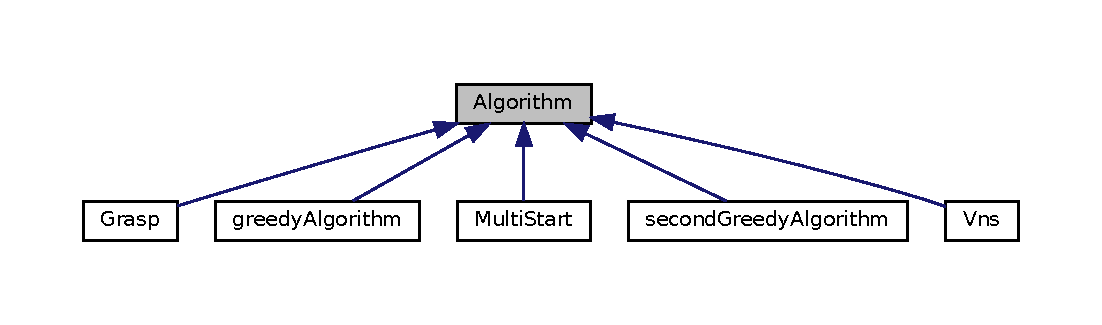
\includegraphics[width=350pt]{classAlgorithm__inherit__graph}
\end{center}
\end{figure}


Collaboration diagram for Algorithm\+:\nopagebreak
\begin{figure}[H]
\begin{center}
\leavevmode
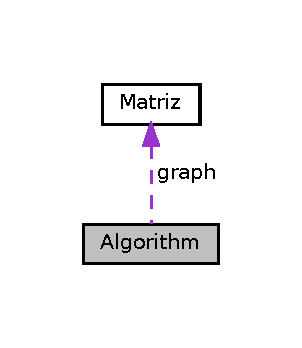
\includegraphics[width=145pt]{classAlgorithm__coll__graph}
\end{center}
\end{figure}
\subsection*{Public Member Functions}
\begin{DoxyCompactItemize}
\item 
\hyperlink{classAlgorithm_a89df1d2c6751f70733f38daa0ee2a13b}{Algorithm} (std\+::string filename)
\begin{DoxyCompactList}\small\item\em Construct a new \hyperlink{classAlgorithm}{Algorithm} object. \end{DoxyCompactList}\item 
virtual std\+::vector$<$ int $>$ \hyperlink{classAlgorithm_af6ea9eb9a6dbd41896e3fd7dabac096b}{execute} ()=0
\begin{DoxyCompactList}\small\item\em Method that executes the algorithm. \end{DoxyCompactList}\end{DoxyCompactItemize}
\subsection*{Protected Attributes}
\begin{DoxyCompactItemize}
\item 
\mbox{\Hypertarget{classAlgorithm_ac738351f4331aee2fb965f689b7be273}\label{classAlgorithm_ac738351f4331aee2fb965f689b7be273}} 
\hyperlink{classMatriz}{Matriz} {\bfseries graph}
\end{DoxyCompactItemize}


\subsection{Detailed Description}
virtual algorithm class used to solve the maxmean problem 

\subsection{Constructor \& Destructor Documentation}
\mbox{\Hypertarget{classAlgorithm_a89df1d2c6751f70733f38daa0ee2a13b}\label{classAlgorithm_a89df1d2c6751f70733f38daa0ee2a13b}} 
\index{Algorithm@{Algorithm}!Algorithm@{Algorithm}}
\index{Algorithm@{Algorithm}!Algorithm@{Algorithm}}
\subsubsection{\texorpdfstring{Algorithm()}{Algorithm()}}
{\footnotesize\ttfamily Algorithm\+::\+Algorithm (\begin{DoxyParamCaption}\item[{std\+::string}]{filename }\end{DoxyParamCaption})\hspace{0.3cm}{\ttfamily [inline]}}



Construct a new \hyperlink{classAlgorithm}{Algorithm} object. 


\begin{DoxyParams}{Parameters}
{\em filename} & \\
\hline
\end{DoxyParams}

\begin{DoxyCode}
35 : graph(filename)\{\};
\end{DoxyCode}
Here is the call graph for this function\+:\nopagebreak
\begin{figure}[H]
\begin{center}
\leavevmode
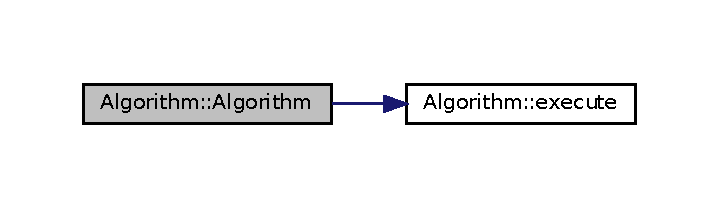
\includegraphics[width=345pt]{classAlgorithm_a89df1d2c6751f70733f38daa0ee2a13b_cgraph}
\end{center}
\end{figure}


\subsection{Member Function Documentation}
\mbox{\Hypertarget{classAlgorithm_af6ea9eb9a6dbd41896e3fd7dabac096b}\label{classAlgorithm_af6ea9eb9a6dbd41896e3fd7dabac096b}} 
\index{Algorithm@{Algorithm}!execute@{execute}}
\index{execute@{execute}!Algorithm@{Algorithm}}
\subsubsection{\texorpdfstring{execute()}{execute()}}
{\footnotesize\ttfamily virtual std\+::vector$<$int$>$ Algorithm\+::execute (\begin{DoxyParamCaption}{ }\end{DoxyParamCaption})\hspace{0.3cm}{\ttfamily [pure virtual]}}



Method that executes the algorithm. 

\begin{DoxyReturn}{Returns}
std\+::vector$<$int$>$ 
\end{DoxyReturn}


Implemented in \hyperlink{classVns_aece2ea2cb74dd3608570321fcbb2de0c}{Vns}, \hyperlink{classGrasp_a335b063bccd26b434dda3a3a69d6d711}{Grasp}, \hyperlink{classMultiStart_a9d842b1f602c4b8a47bf6d88d483ccae}{Multi\+Start}, \hyperlink{classsecondGreedyAlgorithm_a119a730116003d00438179ccf4e2cafd}{second\+Greedy\+Algorithm}, and \hyperlink{classgreedyAlgorithm_a37c81600b24a32ae25b6f0eeab643a7a}{greedy\+Algorithm}.

Here is the caller graph for this function\+:\nopagebreak
\begin{figure}[H]
\begin{center}
\leavevmode
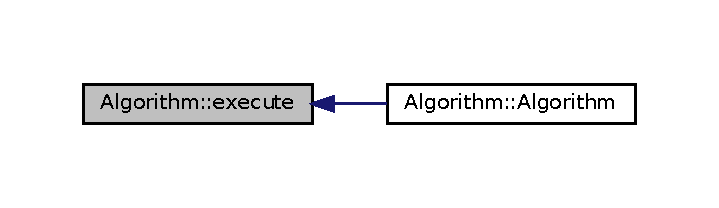
\includegraphics[width=345pt]{classAlgorithm_af6ea9eb9a6dbd41896e3fd7dabac096b_icgraph}
\end{center}
\end{figure}


The documentation for this class was generated from the following file\+:\begin{DoxyCompactItemize}
\item 
include/\hyperlink{algorithm_8hpp}{algorithm.\+hpp}\end{DoxyCompactItemize}

\hypertarget{classGrasp}{}\section{Grasp Class Reference}
\label{classGrasp}\index{Grasp@{Grasp}}


\hyperlink{classGrasp}{Grasp} implementation to solve Max Mean.  




{\ttfamily \#include $<$grasp.\+hpp$>$}



Inheritance diagram for Grasp\+:\nopagebreak
\begin{figure}[H]
\begin{center}
\leavevmode
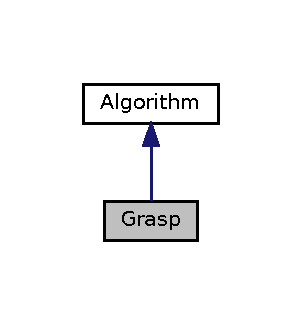
\includegraphics[width=145pt]{classGrasp__inherit__graph}
\end{center}
\end{figure}


Collaboration diagram for Grasp\+:\nopagebreak
\begin{figure}[H]
\begin{center}
\leavevmode
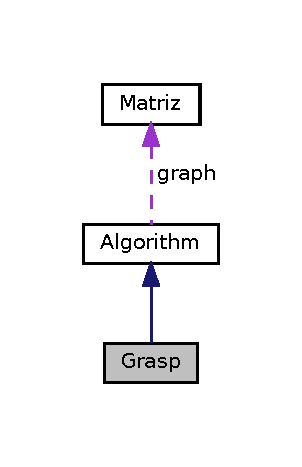
\includegraphics[width=145pt]{classGrasp__coll__graph}
\end{center}
\end{figure}
\subsection*{Public Member Functions}
\begin{DoxyCompactItemize}
\item 
\hyperlink{classGrasp_acf9e8029b833f71283be24a9309c5cad}{Grasp} (std\+::string filename, int iter, int noimprov, bool anx)
\begin{DoxyCompactList}\small\item\em Construct a new \hyperlink{classGrasp}{Grasp} object. \end{DoxyCompactList}\item 
std\+::vector$<$ int $>$ \hyperlink{classGrasp_aef091e71dd747ebcb78e1ebcdcf44221}{construction\+Phase} (std\+::vector$<$ int $>$ first\+Candidates)
\begin{DoxyCompactList}\small\item\em Function to create a initial solution for the problem. \end{DoxyCompactList}\item 
std\+::vector$<$ int $>$ \hyperlink{classGrasp_ac63d4a1892472663549c77686edfed74}{R\+CL} (std\+::vector$<$ int $>$, std\+::vector$<$ int $>$)
\begin{DoxyCompactList}\small\item\em Function to create a R\+CL array based on an initial solution. \end{DoxyCompactList}\item 
std\+::vector$<$ int $>$ \hyperlink{classGrasp_a7c5bebb4a0dea342928f66fb73a56559}{local\+Search} (std\+::vector$<$ int $>$, std\+::vector$<$ int $>$)
\begin{DoxyCompactList}\small\item\em Function that uses a greedy algorithm to improve the solution. \end{DoxyCompactList}\item 
std\+::pair$<$ int, bool $>$ \hyperlink{classGrasp_a858a5aee4066bf5ef7946e8ea3e10bcf}{get\+Worst\+Md} (std\+::vector$<$ int $>$)
\begin{DoxyCompactList}\small\item\em Return the worst node (worst afinity) in the actual solution. \end{DoxyCompactList}\item 
std\+::vector$<$ int $>$ \hyperlink{classGrasp_a335b063bccd26b434dda3a3a69d6d711}{execute} ()
\begin{DoxyCompactList}\small\item\em Method that executes the algorithm. \end{DoxyCompactList}\end{DoxyCompactItemize}
\subsection*{Additional Inherited Members}


\subsection{Detailed Description}
\hyperlink{classGrasp}{Grasp} implementation to solve Max Mean. 

\subsection{Constructor \& Destructor Documentation}
\mbox{\Hypertarget{classGrasp_acf9e8029b833f71283be24a9309c5cad}\label{classGrasp_acf9e8029b833f71283be24a9309c5cad}} 
\index{Grasp@{Grasp}!Grasp@{Grasp}}
\index{Grasp@{Grasp}!Grasp@{Grasp}}
\subsubsection{\texorpdfstring{Grasp()}{Grasp()}}
{\footnotesize\ttfamily Grasp\+::\+Grasp (\begin{DoxyParamCaption}\item[{std\+::string}]{filename,  }\item[{int}]{iter,  }\item[{int}]{noimprov,  }\item[{bool}]{anx }\end{DoxyParamCaption})\hspace{0.3cm}{\ttfamily [inline]}}



Construct a new \hyperlink{classGrasp}{Grasp} object. 


\begin{DoxyParams}{Parameters}
{\em filename} & \\
\hline
{\em iter} & \\
\hline
{\em noimprov} & \\
\hline
{\em anx} & \\
\hline
\end{DoxyParams}

\begin{DoxyCode}
37 : \hyperlink{classAlgorithm_a89df1d2c6751f70733f38daa0ee2a13b}{Algorithm}(filename), Iterations(iter), NoImprov(noimprov), anxious(anx) \{\}
\end{DoxyCode}
Here is the call graph for this function\+:\nopagebreak
\begin{figure}[H]
\begin{center}
\leavevmode
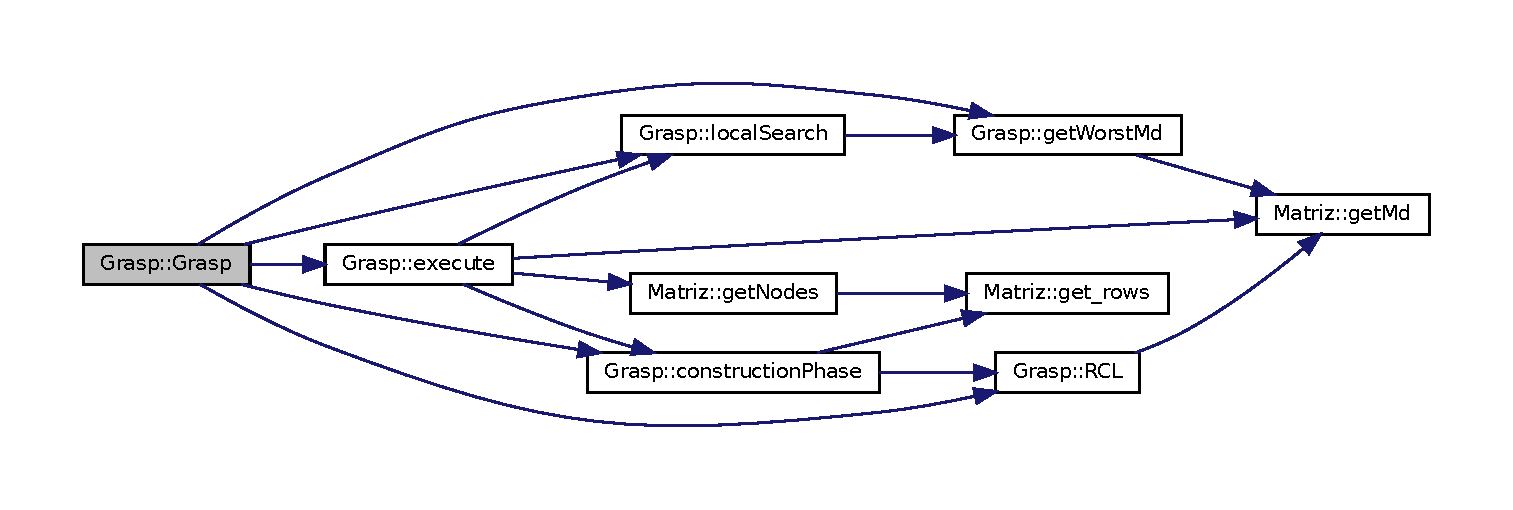
\includegraphics[width=350pt]{classGrasp_acf9e8029b833f71283be24a9309c5cad_cgraph}
\end{center}
\end{figure}


\subsection{Member Function Documentation}
\mbox{\Hypertarget{classGrasp_aef091e71dd747ebcb78e1ebcdcf44221}\label{classGrasp_aef091e71dd747ebcb78e1ebcdcf44221}} 
\index{Grasp@{Grasp}!construction\+Phase@{construction\+Phase}}
\index{construction\+Phase@{construction\+Phase}!Grasp@{Grasp}}
\subsubsection{\texorpdfstring{construction\+Phase()}{constructionPhase()}}
{\footnotesize\ttfamily std\+::vector$<$ int $>$ Grasp\+::construction\+Phase (\begin{DoxyParamCaption}\item[{std\+::vector$<$ int $>$}]{first\+Candidates }\end{DoxyParamCaption})}



Function to create a initial solution for the problem. 


\begin{DoxyParams}{Parameters}
{\em first\+Candidates} & \\
\hline
\end{DoxyParams}
\begin{DoxyReturn}{Returns}
std\+::vector$<$int$>$ 
\end{DoxyReturn}

\begin{DoxyCode}
3                                                                        \{
4    std::vector<int> solution;
5    \textcolor{keywordtype}{int} firstNode = rand() % firstCandidates.size();
6    solution.push\_back(firstCandidates[firstNode]);
7    \textcolor{keywordtype}{int} solutionSize = (rand() % (graph.\hyperlink{classMatriz_a6b18342f8c083baece693ff41185a206}{get\_rows}() - 2)) + 2;
8    \textcolor{keywordflow}{while}(solution.size() < solutionSize) \{
9      std::vector<int> rclVector = \hyperlink{classGrasp_ac63d4a1892472663549c77686edfed74}{RCL}(solution, firstCandidates);
10      solution.push\_back(rclVector[rand() % rclVector.size()]);
11    \}
12    \textcolor{keywordflow}{return} solution;
13  \}
\end{DoxyCode}
Here is the call graph for this function\+:\nopagebreak
\begin{figure}[H]
\begin{center}
\leavevmode
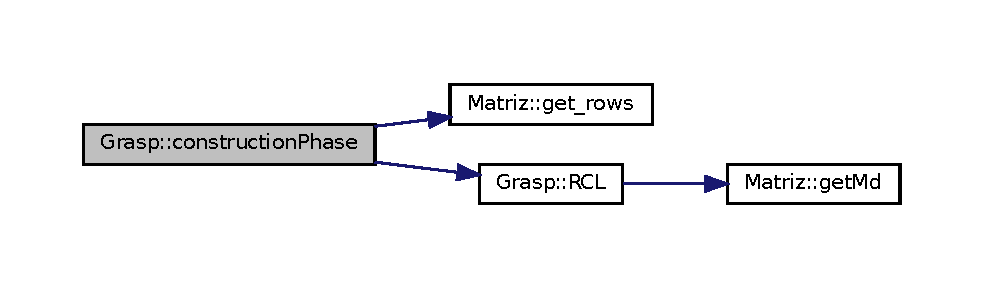
\includegraphics[width=350pt]{classGrasp_aef091e71dd747ebcb78e1ebcdcf44221_cgraph}
\end{center}
\end{figure}
Here is the caller graph for this function\+:\nopagebreak
\begin{figure}[H]
\begin{center}
\leavevmode
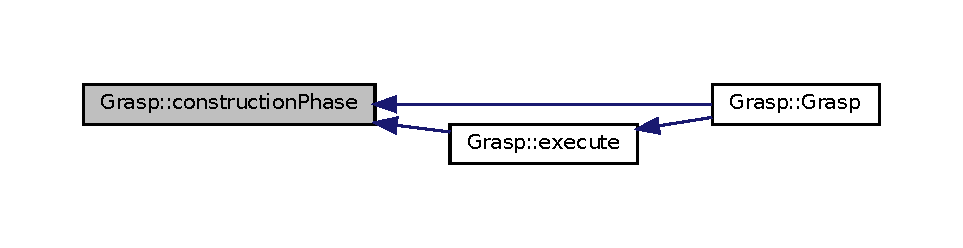
\includegraphics[width=350pt]{classGrasp_aef091e71dd747ebcb78e1ebcdcf44221_icgraph}
\end{center}
\end{figure}
\mbox{\Hypertarget{classGrasp_a335b063bccd26b434dda3a3a69d6d711}\label{classGrasp_a335b063bccd26b434dda3a3a69d6d711}} 
\index{Grasp@{Grasp}!execute@{execute}}
\index{execute@{execute}!Grasp@{Grasp}}
\subsubsection{\texorpdfstring{execute()}{execute()}}
{\footnotesize\ttfamily std\+::vector$<$ int $>$ Grasp\+::execute (\begin{DoxyParamCaption}{ }\end{DoxyParamCaption})\hspace{0.3cm}{\ttfamily [virtual]}}



Method that executes the algorithm. 

\begin{DoxyReturn}{Returns}
std\+::vector$<$int$>$ 
\end{DoxyReturn}


Implements \hyperlink{classAlgorithm_af6ea9eb9a6dbd41896e3fd7dabac096b}{Algorithm}.


\begin{DoxyCode}
82                               \{
83   std::vector<int> firstNodes = graph.\hyperlink{classMatriz_a394b84a5ec13fd2f4d202ab218680afe}{getNodes}();
84   std::vector<int> bestSolution;
85   bestSolution.push\_back(0);
86   \textcolor{keywordtype}{float} bestDistance = graph.\hyperlink{classMatriz_a8df14a27d791f24206dd633b2a685c5b}{getMd}(bestSolution);
87   \textcolor{keywordtype}{int} iterations = 0;
88   \textcolor{keywordtype}{int} noImprovement = 0;
89   \textcolor{keywordflow}{while}(iterations < this->Iterations && noImprovement < this->NoImprov) \{
90     iterations++;
91     std::vector<int> initialSol = \hyperlink{classGrasp_aef091e71dd747ebcb78e1ebcdcf44221}{constructionPhase}(firstNodes);
92     std::vector<int> localSearchVector = \hyperlink{classGrasp_a7c5bebb4a0dea342928f66fb73a56559}{localSearch}(initialSol, firstNodes);
93     \textcolor{keywordtype}{float} testMd = graph.\hyperlink{classMatriz_a8df14a27d791f24206dd633b2a685c5b}{getMd}(localSearchVector);
94     \textcolor{keywordflow}{if}(testMd > bestDistance) \{
95       bestSolution = localSearchVector;
96       bestDistance = testMd;
97       noImprovement = 0;
98     \} \textcolor{keywordflow}{else} \{
99       noImprovement++;
100     \}
101   \}
102   
103 \textcolor{keywordflow}{return} bestSolution;
104 \}
\end{DoxyCode}
Here is the call graph for this function\+:\nopagebreak
\begin{figure}[H]
\begin{center}
\leavevmode
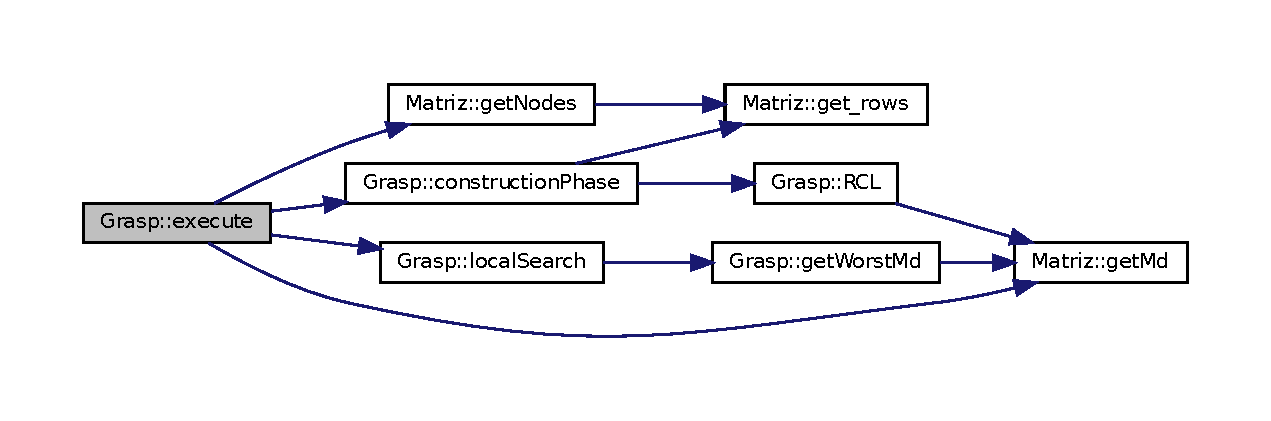
\includegraphics[width=350pt]{classGrasp_a335b063bccd26b434dda3a3a69d6d711_cgraph}
\end{center}
\end{figure}
Here is the caller graph for this function\+:\nopagebreak
\begin{figure}[H]
\begin{center}
\leavevmode
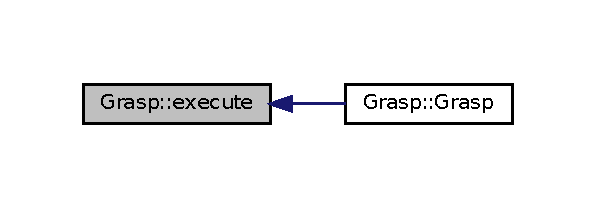
\includegraphics[width=286pt]{classGrasp_a335b063bccd26b434dda3a3a69d6d711_icgraph}
\end{center}
\end{figure}
\mbox{\Hypertarget{classGrasp_a858a5aee4066bf5ef7946e8ea3e10bcf}\label{classGrasp_a858a5aee4066bf5ef7946e8ea3e10bcf}} 
\index{Grasp@{Grasp}!get\+Worst\+Md@{get\+Worst\+Md}}
\index{get\+Worst\+Md@{get\+Worst\+Md}!Grasp@{Grasp}}
\subsubsection{\texorpdfstring{get\+Worst\+Md()}{getWorstMd()}}
{\footnotesize\ttfamily std\+::pair$<$ int, bool $>$ Grasp\+::get\+Worst\+Md (\begin{DoxyParamCaption}\item[{std\+::vector$<$ int $>$}]{solution }\end{DoxyParamCaption})}



Return the worst node (worst afinity) in the actual solution. 

\begin{DoxyReturn}{Returns}
std\+::pair$<$int,bool$>$ 
\end{DoxyReturn}

\begin{DoxyCode}
53                                                            \{
54   std::vector<std::pair<int, bool>> vertexVector;
55   std::pair<int, bool> vertex(-1, \textcolor{keyword}{false});
56   vertexVector.push\_back(vertex);
57   \textcolor{keywordtype}{float} currentDistance = graph.\hyperlink{classMatriz_a8df14a27d791f24206dd633b2a685c5b}{getMd}(solution);
58   \textcolor{keywordtype}{float} currentEdgeSum = currentDistance * solution.size();
59   \textcolor{keywordflow}{for} (\textcolor{keywordtype}{int} i = 0; i < solution.size(); i++)
60   \{
61     \textcolor{keywordtype}{int} vertex = solution[i];
62     solution.erase(solution.begin() + i);
63     \textcolor{keywordtype}{float} nextMd = graph.\hyperlink{classMatriz_a8df14a27d791f24206dd633b2a685c5b}{getMd}(solution);
64     solution.insert(solution.begin() + i, vertex);
65     \textcolor{keywordflow}{if} (nextMd > currentDistance)
66     \{
67       \textcolor{keywordflow}{if}(anxious) \{
68         \textcolor{keywordflow}{return} std::pair<int,bool>(i,\textcolor{keyword}{true});;
69       \}
70       currentDistance = nextMd;
71       vertexVector.clear();
72       vertexVector.push\_back(std::pair<int, bool>(i, \textcolor{keyword}{true}));
73     \}
74     \textcolor{keywordflow}{else} \textcolor{keywordflow}{if} (nextMd == currentDistance)
75     \{
76       vertexVector.push\_back(std::pair<int, bool>(i, \textcolor{keyword}{true}));
77     \}
78   \}
79   \textcolor{keywordflow}{return} vertexVector[rand() % vertexVector.size()];
80 \}
\end{DoxyCode}
Here is the call graph for this function\+:\nopagebreak
\begin{figure}[H]
\begin{center}
\leavevmode
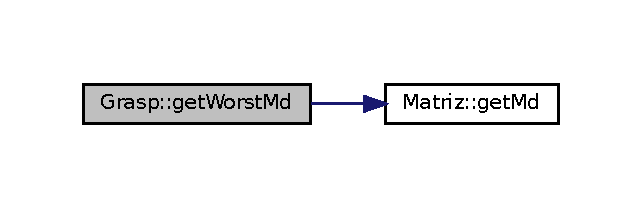
\includegraphics[width=308pt]{classGrasp_a858a5aee4066bf5ef7946e8ea3e10bcf_cgraph}
\end{center}
\end{figure}
Here is the caller graph for this function\+:\nopagebreak
\begin{figure}[H]
\begin{center}
\leavevmode
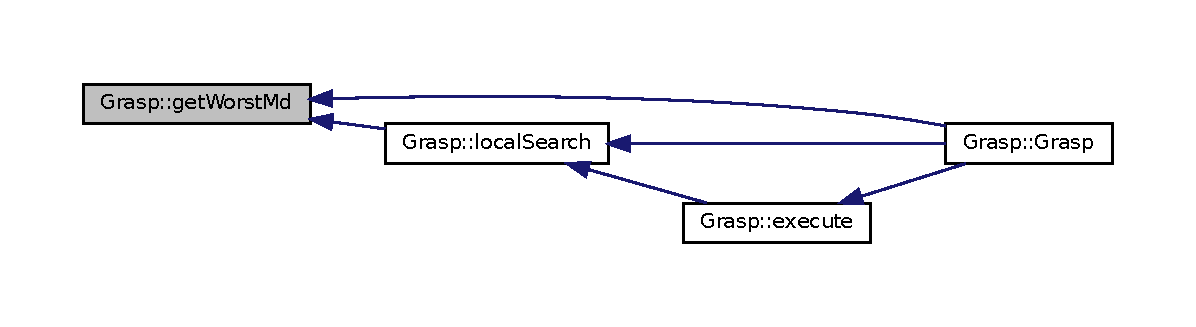
\includegraphics[width=350pt]{classGrasp_a858a5aee4066bf5ef7946e8ea3e10bcf_icgraph}
\end{center}
\end{figure}
\mbox{\Hypertarget{classGrasp_a7c5bebb4a0dea342928f66fb73a56559}\label{classGrasp_a7c5bebb4a0dea342928f66fb73a56559}} 
\index{Grasp@{Grasp}!local\+Search@{local\+Search}}
\index{local\+Search@{local\+Search}!Grasp@{Grasp}}
\subsubsection{\texorpdfstring{local\+Search()}{localSearch()}}
{\footnotesize\ttfamily std\+::vector$<$ int $>$ Grasp\+::local\+Search (\begin{DoxyParamCaption}\item[{std\+::vector$<$ int $>$}]{solution,  }\item[{std\+::vector$<$ int $>$}]{first\+Candidates }\end{DoxyParamCaption})}



Function that uses a greedy algorithm to improve the solution. 

\begin{DoxyReturn}{Returns}
std\+::vector$<$int$>$ 
\end{DoxyReturn}

\begin{DoxyCode}
40                                                                                          \{
41   \textcolor{keywordtype}{bool} improvement = \textcolor{keyword}{true};
42   \textcolor{keywordflow}{while}(improvement) \{
43     improvement = \textcolor{keyword}{false};
44     std::pair<int,bool> worst = \hyperlink{classGrasp_a858a5aee4066bf5ef7946e8ea3e10bcf}{getWorstMd}(solution);
45     \textcolor{keywordflow}{if}(worst.second)\{
46       improvement = \textcolor{keyword}{true};
47       solution.erase(solution.begin() + worst.first);
48     \}
49   \}
50   \textcolor{keywordflow}{return} solution;
51 \}
\end{DoxyCode}
Here is the call graph for this function\+:\nopagebreak
\begin{figure}[H]
\begin{center}
\leavevmode
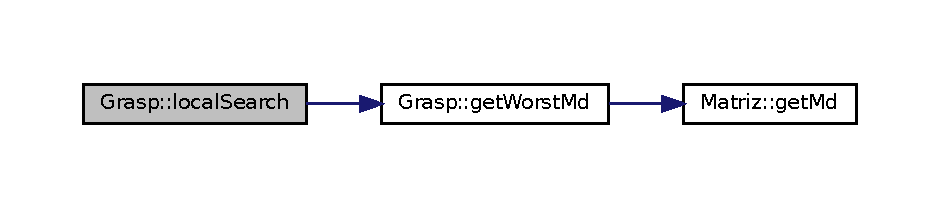
\includegraphics[width=350pt]{classGrasp_a7c5bebb4a0dea342928f66fb73a56559_cgraph}
\end{center}
\end{figure}
Here is the caller graph for this function\+:\nopagebreak
\begin{figure}[H]
\begin{center}
\leavevmode
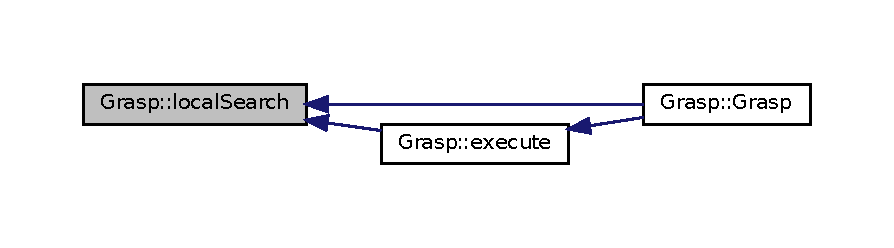
\includegraphics[width=350pt]{classGrasp_a7c5bebb4a0dea342928f66fb73a56559_icgraph}
\end{center}
\end{figure}
\mbox{\Hypertarget{classGrasp_ac63d4a1892472663549c77686edfed74}\label{classGrasp_ac63d4a1892472663549c77686edfed74}} 
\index{Grasp@{Grasp}!R\+CL@{R\+CL}}
\index{R\+CL@{R\+CL}!Grasp@{Grasp}}
\subsubsection{\texorpdfstring{R\+C\+L()}{RCL()}}
{\footnotesize\ttfamily std\+::vector$<$ int $>$ Grasp\+::\+R\+CL (\begin{DoxyParamCaption}\item[{std\+::vector$<$ int $>$}]{solution,  }\item[{std\+::vector$<$ int $>$}]{first\+Candidates }\end{DoxyParamCaption})}



Function to create a R\+CL array based on an initial solution. 

\begin{DoxyReturn}{Returns}
std\+::vector$<$int$>$ 
\end{DoxyReturn}

\begin{DoxyCode}
15                                                                                   \{
16    std::vector<int> sortedNodes;
17    std::vector<float> sortedDistances;
18    std::vector<int> rclVector;
19    \textcolor{keywordflow}{for}(\textcolor{keywordtype}{int} i = 0; i < firstCandidates.size(); i++) \{
20      \textcolor{keywordflow}{if}(std::find(solution.begin(), solution.end(), firstCandidates[i]) == solution.end()) \{
21        solution.push\_back(firstCandidates[i]);
22        \textcolor{keywordtype}{float} testMd = graph.\hyperlink{classMatriz_a8df14a27d791f24206dd633b2a685c5b}{getMd}(solution);
23        solution.pop\_back();
24        \textcolor{keywordtype}{int} position = 0;
25        \textcolor{keywordflow}{for}(\textcolor{keywordtype}{int} j = 0; j < sortedDistances.size(); j++) \{
26          \textcolor{keywordflow}{if}(testMd < sortedDistances[j]) \{
27            position++;
28          \}
29        \}
30        sortedDistances.insert(sortedDistances.begin() + position, testMd);
31        sortedNodes.insert(sortedNodes.begin() + position, firstCandidates[i]);
32      \}
33    \}
34    \textcolor{keywordtype}{int} percent = (sortedNodes.size() / (1 / 0.2));
35    percent = percent == 0 ? 1 : percent;
36    std::copy(sortedNodes.begin(), sortedNodes.begin() + percent, std::back\_inserter(rclVector));
37    \textcolor{keywordflow}{return} rclVector;
38  \}
\end{DoxyCode}
Here is the call graph for this function\+:\nopagebreak
\begin{figure}[H]
\begin{center}
\leavevmode
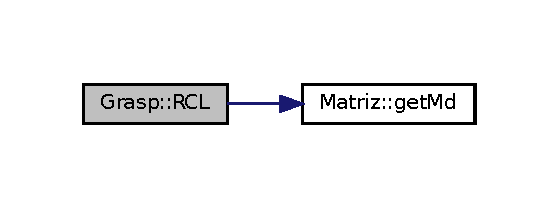
\includegraphics[width=268pt]{classGrasp_ac63d4a1892472663549c77686edfed74_cgraph}
\end{center}
\end{figure}
Here is the caller graph for this function\+:\nopagebreak
\begin{figure}[H]
\begin{center}
\leavevmode
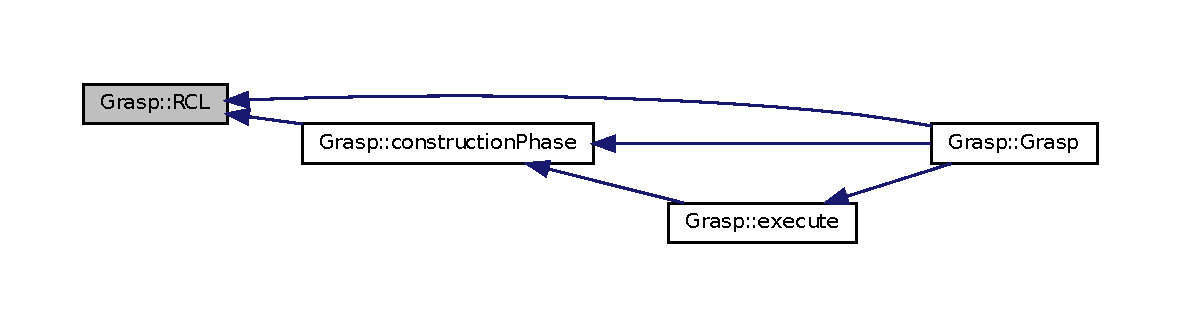
\includegraphics[width=350pt]{classGrasp_ac63d4a1892472663549c77686edfed74_icgraph}
\end{center}
\end{figure}


The documentation for this class was generated from the following files\+:\begin{DoxyCompactItemize}
\item 
include/\hyperlink{grasp_8hpp}{grasp.\+hpp}\item 
src/grasp.\+cpp\end{DoxyCompactItemize}

\hypertarget{classgreedyAlgorithm}{}\section{greedy\+Algorithm Class Reference}
\label{classgreedyAlgorithm}\index{greedy\+Algorithm@{greedy\+Algorithm}}


Implementation of the greedy algorithm to solve Max Mean problem.  




{\ttfamily \#include $<$greedy\+Algorithm.\+hpp$>$}



Inheritance diagram for greedy\+Algorithm\+:
\nopagebreak
\begin{figure}[H]
\begin{center}
\leavevmode
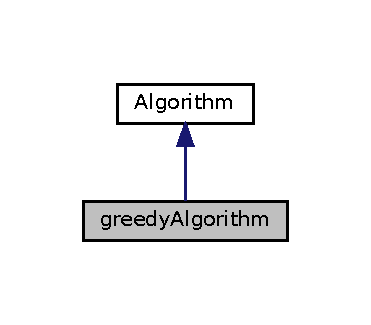
\includegraphics[width=178pt]{classgreedyAlgorithm__inherit__graph}
\end{center}
\end{figure}


Collaboration diagram for greedy\+Algorithm\+:
\nopagebreak
\begin{figure}[H]
\begin{center}
\leavevmode
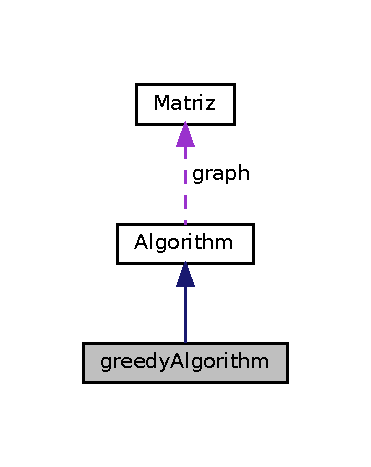
\includegraphics[width=178pt]{classgreedyAlgorithm__coll__graph}
\end{center}
\end{figure}
\subsection*{Public Member Functions}
\begin{DoxyCompactItemize}
\item 
\hyperlink{classgreedyAlgorithm_acd4c3a073c8ed2e93bbf402363ebd71d}{greedy\+Algorithm} (std\+::string filename)
\begin{DoxyCompactList}\small\item\em Construct a new greedy \hyperlink{classAlgorithm}{Algorithm} object. \end{DoxyCompactList}\item 
std\+::vector$<$ int $>$ \hyperlink{classgreedyAlgorithm_a37c81600b24a32ae25b6f0eeab643a7a}{execute} ()
\begin{DoxyCompactList}\small\item\em Method that executes the algorithm. \end{DoxyCompactList}\item 
std\+::pair$<$ int, bool $>$ \hyperlink{classgreedyAlgorithm_a4968e1371d2fdfb1b1b6f24b57dd1f07}{maximize\+Md} (std\+::vector$<$ int $>$ solution)
\begin{DoxyCompactList}\small\item\em Returns the node with the max mean dispersion. \end{DoxyCompactList}\end{DoxyCompactItemize}
\subsection*{Additional Inherited Members}


\subsection{Detailed Description}
Implementation of the greedy algorithm to solve Max Mean problem. 

\subsection{Constructor \& Destructor Documentation}
\mbox{\Hypertarget{classgreedyAlgorithm_acd4c3a073c8ed2e93bbf402363ebd71d}\label{classgreedyAlgorithm_acd4c3a073c8ed2e93bbf402363ebd71d}} 
\index{greedy\+Algorithm@{greedy\+Algorithm}!greedy\+Algorithm@{greedy\+Algorithm}}
\index{greedy\+Algorithm@{greedy\+Algorithm}!greedy\+Algorithm@{greedy\+Algorithm}}
\subsubsection{\texorpdfstring{greedy\+Algorithm()}{greedyAlgorithm()}}
{\footnotesize\ttfamily greedy\+Algorithm\+::greedy\+Algorithm (\begin{DoxyParamCaption}\item[{std\+::string}]{filename }\end{DoxyParamCaption})\hspace{0.3cm}{\ttfamily [inline]}}



Construct a new greedy \hyperlink{classAlgorithm}{Algorithm} object. 


\begin{DoxyParams}{Parameters}
{\em filename} & \\
\hline
\end{DoxyParams}

\begin{DoxyCode}
30 : \hyperlink{classAlgorithm_a89df1d2c6751f70733f38daa0ee2a13b}{Algorithm}(filename) \{\}
\end{DoxyCode}
Here is the call graph for this function\+:
\nopagebreak
\begin{figure}[H]
\begin{center}
\leavevmode
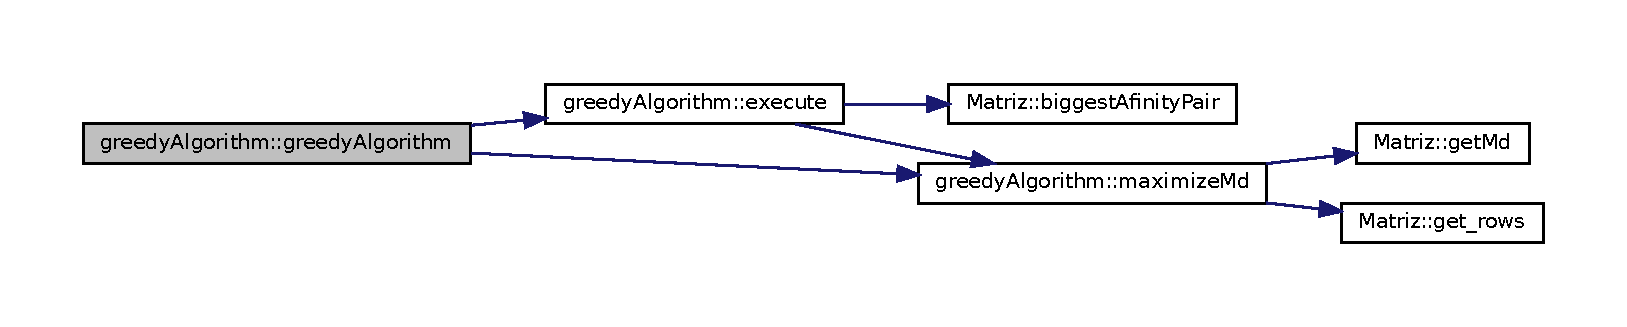
\includegraphics[width=350pt]{classgreedyAlgorithm_acd4c3a073c8ed2e93bbf402363ebd71d_cgraph}
\end{center}
\end{figure}


\subsection{Member Function Documentation}
\mbox{\Hypertarget{classgreedyAlgorithm_a37c81600b24a32ae25b6f0eeab643a7a}\label{classgreedyAlgorithm_a37c81600b24a32ae25b6f0eeab643a7a}} 
\index{greedy\+Algorithm@{greedy\+Algorithm}!execute@{execute}}
\index{execute@{execute}!greedy\+Algorithm@{greedy\+Algorithm}}
\subsubsection{\texorpdfstring{execute()}{execute()}}
{\footnotesize\ttfamily std\+::vector$<$ int $>$ greedy\+Algorithm\+::execute (\begin{DoxyParamCaption}{ }\end{DoxyParamCaption})\hspace{0.3cm}{\ttfamily [virtual]}}



Method that executes the algorithm. 

\begin{DoxyReturn}{Returns}
std\+::vector$<$int$>$ 
\end{DoxyReturn}


Implements \hyperlink{classAlgorithm_af6ea9eb9a6dbd41896e3fd7dabac096b}{Algorithm}.


\begin{DoxyCode}
4 \{
5   std::vector<int> solution;
6   std::pair<int, int> firstSolutionPair = graph.\hyperlink{classMatriz_a30e8aba7a2868aaa98f11d3037ff8319}{biggestAfinityPair}();
7   solution.push\_back(firstSolutionPair.first);
8   solution.push\_back(firstSolutionPair.second);
9   std::pair<int, bool> k = \hyperlink{classgreedyAlgorithm_a4968e1371d2fdfb1b1b6f24b57dd1f07}{maximizeMd}(solution);
10   \textcolor{keywordflow}{while} (k.second)
11   \{
12     solution.push\_back(k.first);
13     k = \hyperlink{classgreedyAlgorithm_a4968e1371d2fdfb1b1b6f24b57dd1f07}{maximizeMd}(solution);
14   \}
15   \textcolor{keywordflow}{return} solution;
16 \}
\end{DoxyCode}
Here is the call graph for this function\+:
\nopagebreak
\begin{figure}[H]
\begin{center}
\leavevmode
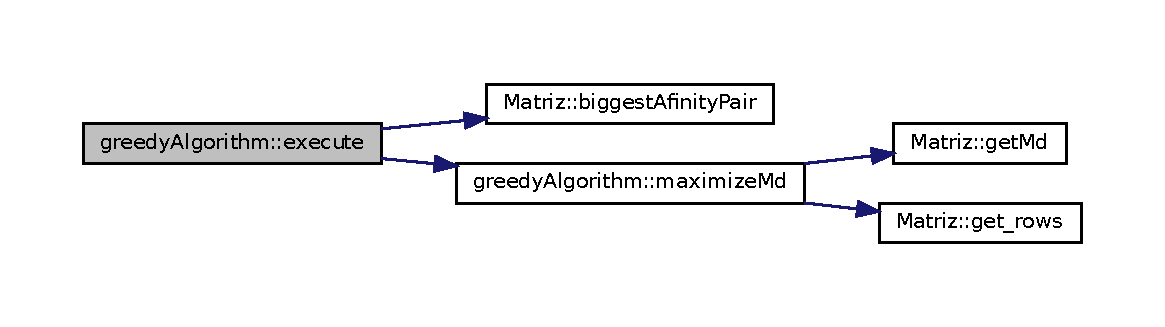
\includegraphics[width=350pt]{classgreedyAlgorithm_a37c81600b24a32ae25b6f0eeab643a7a_cgraph}
\end{center}
\end{figure}
Here is the caller graph for this function\+:
\nopagebreak
\begin{figure}[H]
\begin{center}
\leavevmode
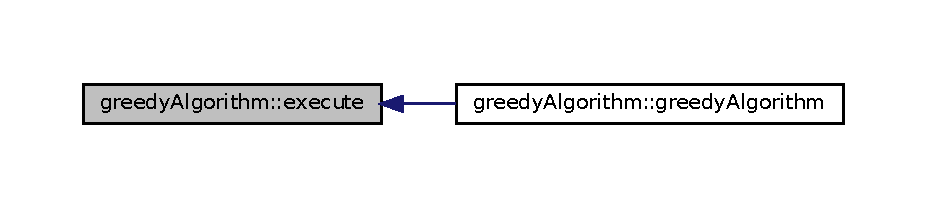
\includegraphics[width=350pt]{classgreedyAlgorithm_a37c81600b24a32ae25b6f0eeab643a7a_icgraph}
\end{center}
\end{figure}
\mbox{\Hypertarget{classgreedyAlgorithm_a4968e1371d2fdfb1b1b6f24b57dd1f07}\label{classgreedyAlgorithm_a4968e1371d2fdfb1b1b6f24b57dd1f07}} 
\index{greedy\+Algorithm@{greedy\+Algorithm}!maximize\+Md@{maximize\+Md}}
\index{maximize\+Md@{maximize\+Md}!greedy\+Algorithm@{greedy\+Algorithm}}
\subsubsection{\texorpdfstring{maximize\+Md()}{maximizeMd()}}
{\footnotesize\ttfamily std\+::pair$<$ int, bool $>$ greedy\+Algorithm\+::maximize\+Md (\begin{DoxyParamCaption}\item[{std\+::vector$<$ int $>$}]{solution }\end{DoxyParamCaption})}



Returns the node with the max mean dispersion. 


\begin{DoxyParams}{Parameters}
{\em solution} & \\
\hline
\end{DoxyParams}
\begin{DoxyReturn}{Returns}
std\+::pair$<$int, bool$>$ 
\end{DoxyReturn}

\begin{DoxyCode}
19 \{
20   std::vector<std::pair<int, bool>> vertexVector;
21   std::pair<int, bool> vertex(-1, \textcolor{keyword}{false});
22   vertexVector.push\_back(vertex);
23   \textcolor{keywordtype}{float} currentDistance = graph.\hyperlink{classMatriz_a8df14a27d791f24206dd633b2a685c5b}{getMd}(solution);
24   \textcolor{keywordflow}{for} (\textcolor{keywordtype}{int} i = 0; i < graph.\hyperlink{classMatriz_a6b18342f8c083baece693ff41185a206}{get\_rows}(); i++)
25   \{
26     \textcolor{keywordflow}{if} (!(std::find(solution.begin(), solution.end(), i) != solution.end()))
27     \{
28       solution.push\_back(i);
29       \textcolor{keywordtype}{float} nextMd = graph.\hyperlink{classMatriz_a8df14a27d791f24206dd633b2a685c5b}{getMd}(solution);
30       solution.pop\_back();
31       \textcolor{keywordflow}{if} (nextMd > currentDistance)
32       \{
33         currentDistance = nextMd;
34         vertexVector.clear();
35         vertexVector.push\_back(std::pair<int, bool>(i, \textcolor{keyword}{true}));
36       \}
37       \textcolor{keywordflow}{else} \textcolor{keywordflow}{if} (nextMd == currentDistance)
38       \{
39         vertexVector.push\_back(std::pair<int, bool>(i, \textcolor{keyword}{true}));
40       \}
41     \}
42   \}
43   \textcolor{keywordflow}{return} vertexVector[rand() % vertexVector.size()];
44 \}
\end{DoxyCode}
Here is the call graph for this function\+:
\nopagebreak
\begin{figure}[H]
\begin{center}
\leavevmode
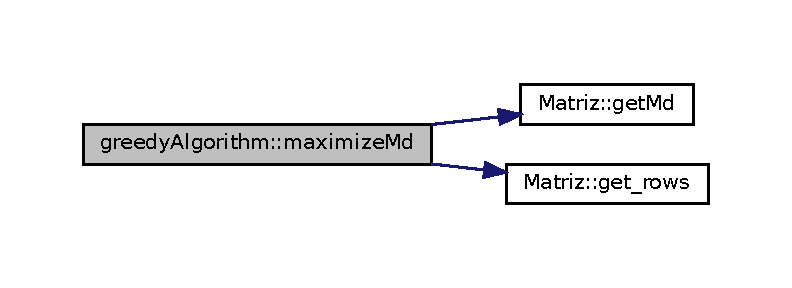
\includegraphics[width=350pt]{classgreedyAlgorithm_a4968e1371d2fdfb1b1b6f24b57dd1f07_cgraph}
\end{center}
\end{figure}
Here is the caller graph for this function\+:
\nopagebreak
\begin{figure}[H]
\begin{center}
\leavevmode
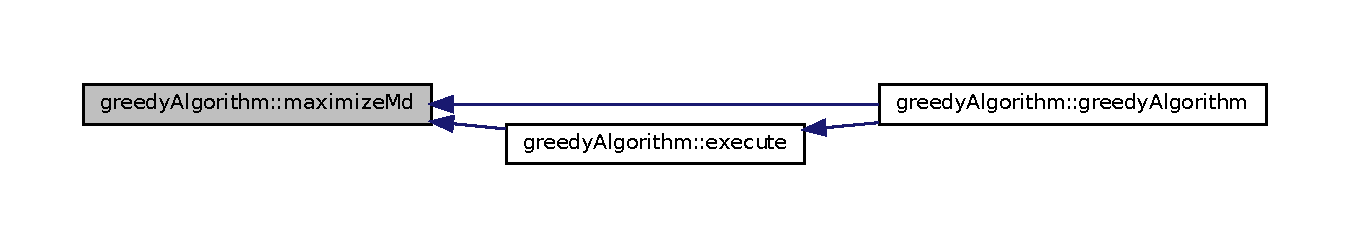
\includegraphics[width=350pt]{classgreedyAlgorithm_a4968e1371d2fdfb1b1b6f24b57dd1f07_icgraph}
\end{center}
\end{figure}


The documentation for this class was generated from the following files\+:\begin{DoxyCompactItemize}
\item 
include/\hyperlink{greedyAlgorithm_8hpp}{greedy\+Algorithm.\+hpp}\item 
src/greedy\+Algorithm.\+cpp\end{DoxyCompactItemize}

\hypertarget{classMatriz}{}\section{Matriz Class Reference}
\label{classMatriz}\index{Matriz@{Matriz}}


Matrix containing all the distances between nodes.  




{\ttfamily \#include $<$matrix.\+hpp$>$}

\subsection*{Public Member Functions}
\begin{DoxyCompactItemize}
\item 
\hyperlink{classMatriz_a388709cfee356a0c78b66e3f538e9318}{Matriz} (std\+::string filename)
\begin{DoxyCompactList}\small\item\em Construct a new \hyperlink{classMatriz}{Matriz} object. \end{DoxyCompactList}\item 
void \hyperlink{classMatriz_aa929f933e9088dc0efecaa9a46d555d9}{resize\+Matrix} (int rows, int cols)
\begin{DoxyCompactList}\small\item\em Change the matrix\textquotesingle{}s dimensions. \end{DoxyCompactList}\item 
int \hyperlink{classMatriz_a6b18342f8c083baece693ff41185a206}{get\+\_\+rows} ()
\begin{DoxyCompactList}\small\item\em Get the rows object. \end{DoxyCompactList}\item 
int \hyperlink{classMatriz_ad6915f9b31f93230a3ce05d01d23a47b}{get\+\_\+cols} ()
\begin{DoxyCompactList}\small\item\em Get the cols object. \end{DoxyCompactList}\item 
void \hyperlink{classMatriz_a71fea2383ce785254c2f27da25ef70c8}{set\+\_\+position} (int row, int col, int value)
\begin{DoxyCompactList}\small\item\em Set the position object. \end{DoxyCompactList}\item 
int \hyperlink{classMatriz_a1894d8447d3ae6992a43e46f93422b88}{get\+\_\+position} (int row, int col)
\begin{DoxyCompactList}\small\item\em Get the position object. \end{DoxyCompactList}\item 
\mbox{\Hypertarget{classMatriz_ae0fd5f42c3797c8d4b85c1d6701e0e7e}\label{classMatriz_ae0fd5f42c3797c8d4b85c1d6701e0e7e}} 
void \hyperlink{classMatriz_ae0fd5f42c3797c8d4b85c1d6701e0e7e}{write} ()
\begin{DoxyCompactList}\small\item\em Print the matrix. \end{DoxyCompactList}\item 
std\+::vector$<$ int $>$ \& \hyperlink{classMatriz_ad2adc857ff1738ebfb7fe42de408737b}{operator\mbox{[}$\,$\mbox{]}} (int index)
\begin{DoxyCompactList}\small\item\em Operator \mbox{[}\mbox{]} overload. \end{DoxyCompactList}\item 
std\+::pair$<$ int, int $>$ \hyperlink{classMatriz_a30e8aba7a2868aaa98f11d3037ff8319}{biggest\+Afinity\+Pair} ()
\begin{DoxyCompactList}\small\item\em returns a pair with the two nodes with the highest afinity \end{DoxyCompactList}\item 
std\+::vector$<$ std\+::pair$<$ int, int $>$ $>$ \hyperlink{classMatriz_a2867d653d30b7fd8ca13e683bd7b8de6}{biggest\+Afinity} ()
\begin{DoxyCompactList}\small\item\em returns a vector of pairs that contains the nodes that have highest afinity \end{DoxyCompactList}\item 
float \hyperlink{classMatriz_a8df14a27d791f24206dd633b2a685c5b}{get\+Md} (std\+::vector$<$ int $>$ solution)
\begin{DoxyCompactList}\small\item\em Returns the mean dispersion. \end{DoxyCompactList}\item 
float \hyperlink{classMatriz_a61efbcc7ea661059ed0dfad32b5273cf}{get\+Md\+Pair} (std\+::vector$<$ std\+::pair$<$ int, int $>$$>$ solution)
\begin{DoxyCompactList}\small\item\em Returns the mean dispersion. \end{DoxyCompactList}\item 
std\+::vector$<$ int $>$ \hyperlink{classMatriz_a394b84a5ec13fd2f4d202ab218680afe}{get\+Nodes} ()
\begin{DoxyCompactList}\small\item\em Returns a vector with all the nodes. \end{DoxyCompactList}\end{DoxyCompactItemize}


\subsection{Detailed Description}
Matrix containing all the distances between nodes. 

\subsection{Constructor \& Destructor Documentation}
\mbox{\Hypertarget{classMatriz_a388709cfee356a0c78b66e3f538e9318}\label{classMatriz_a388709cfee356a0c78b66e3f538e9318}} 
\index{Matriz@{Matriz}!Matriz@{Matriz}}
\index{Matriz@{Matriz}!Matriz@{Matriz}}
\subsubsection{\texorpdfstring{Matriz()}{Matriz()}}
{\footnotesize\ttfamily Matriz\+::\+Matriz (\begin{DoxyParamCaption}\item[{std\+::string}]{filename }\end{DoxyParamCaption})\hspace{0.3cm}{\ttfamily [inline]}}



Construct a new \hyperlink{classMatriz}{Matriz} object. 


\begin{DoxyParams}{Parameters}
{\em \{std\+::string\}} & filename \\
\hline
\end{DoxyParams}

\begin{DoxyCode}
36                              : matrix(0, std::vector<int>(0))
37   \{
38     std::ifstream myFile;
39     myFile.open(filename);
40     \textcolor{keywordtype}{int} numeroVertices = 0;
41     \textcolor{keywordtype}{int} valores = 0;
42     \textcolor{keywordflow}{if} (myFile.is\_open())
43     \{
44       myFile >> numeroVertices;
45     \}
46     this->\hyperlink{classMatriz_aa929f933e9088dc0efecaa9a46d555d9}{resizeMatrix}(numeroVertices, numeroVertices);
47     \textcolor{keywordflow}{for} (\textcolor{keywordtype}{int} i = 0; i < numeroVertices; i++)
48     \{
49       \textcolor{keywordflow}{for} (\textcolor{keywordtype}{int} j = 0; j < numeroVertices; j++)
50       \{
51         matrix[i][j] = 0;
52       \}
53     \}
54     \textcolor{keywordflow}{for} (\textcolor{keywordtype}{int} i = 0; i < numeroVertices; i++)
55     \{
56       \textcolor{keywordflow}{for} (\textcolor{keywordtype}{int} j = 0; j < numeroVertices; j++)
57       \{
58         \textcolor{keywordflow}{if} (!myFile.eof() && matrix[i][j] == 0 && i != j)
59         \{
60           myFile >> valores;
61           matrix[i][j] = valores;
62           matrix[j][i] = valores;
63         \}
64       \}
65     \}
66     myFile.close();
67   \}
\end{DoxyCode}
Here is the call graph for this function\+:\nopagebreak
\begin{figure}[H]
\begin{center}
\leavevmode
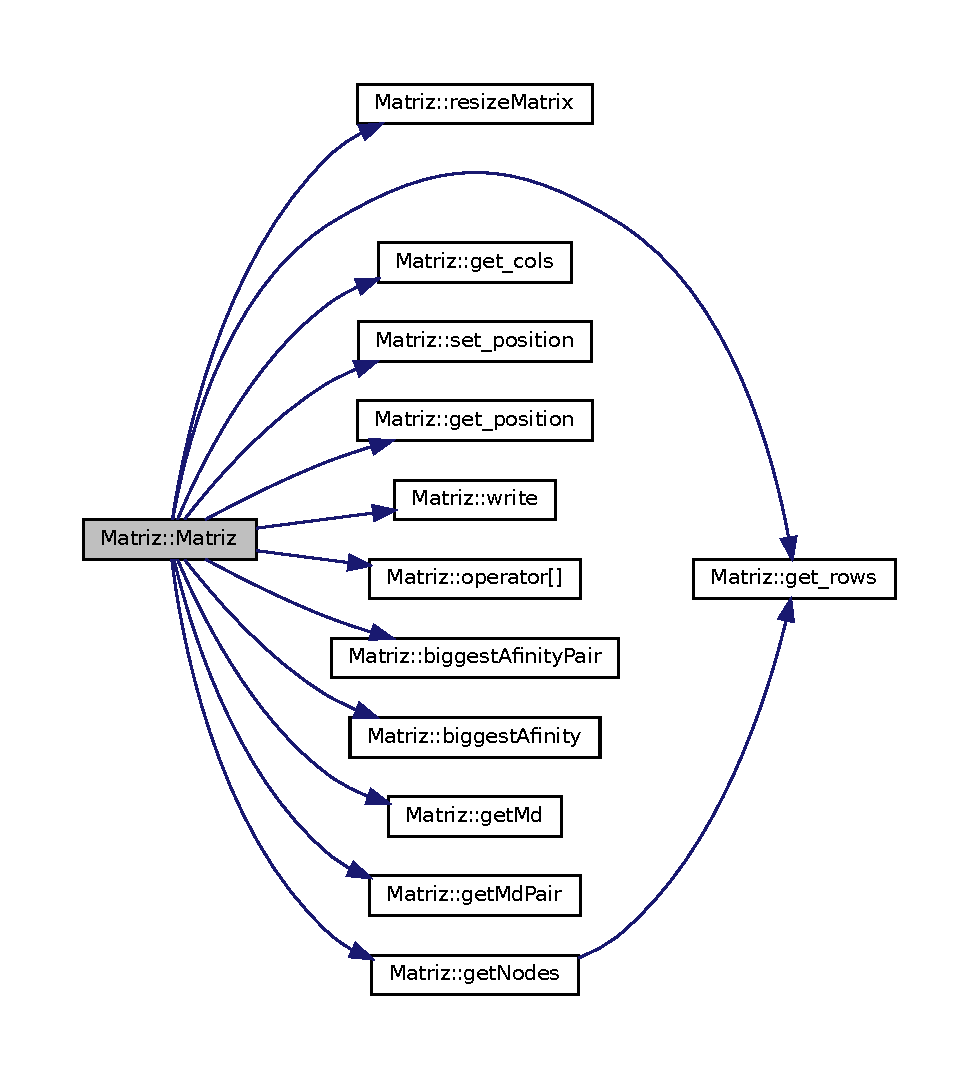
\includegraphics[width=350pt]{classMatriz_a388709cfee356a0c78b66e3f538e9318_cgraph}
\end{center}
\end{figure}


\subsection{Member Function Documentation}
\mbox{\Hypertarget{classMatriz_a2867d653d30b7fd8ca13e683bd7b8de6}\label{classMatriz_a2867d653d30b7fd8ca13e683bd7b8de6}} 
\index{Matriz@{Matriz}!biggest\+Afinity@{biggest\+Afinity}}
\index{biggest\+Afinity@{biggest\+Afinity}!Matriz@{Matriz}}
\subsubsection{\texorpdfstring{biggest\+Afinity()}{biggestAfinity()}}
{\footnotesize\ttfamily std\+::vector$<$ std\+::pair$<$ int, int $>$ $>$ Matriz\+::biggest\+Afinity (\begin{DoxyParamCaption}{ }\end{DoxyParamCaption})}



returns a vector of pairs that contains the nodes that have highest afinity 

\begin{DoxyReturn}{Returns}
std\+::vector$<$std\+::pair$<$int,int$>$$>$ 
\end{DoxyReturn}

\begin{DoxyCode}
98 \{
99   \textcolor{keywordtype}{float} biggestValue = 0;
100   std::vector<std::pair<int, int>> vectorAfinity;
101   \textcolor{keywordflow}{for} (\textcolor{keywordtype}{int} i = 0; i < matrix.size(); i++)
102   \{
103     \textcolor{keywordflow}{for} (\textcolor{keywordtype}{int} j = i + 1; j < matrix.size(); j++)
104     \{
105       \textcolor{keywordflow}{if} (matrix[i][j] >= biggestValue)
106       \{
107         biggestValue = matrix[i][j];
108       \}
109     \}
110   \}
111   \textcolor{keywordflow}{for} (\textcolor{keywordtype}{int} i = 0; i < matrix.size(); i++)
112   \{
113     \textcolor{keywordflow}{for} (\textcolor{keywordtype}{int} j = i + 1; j < matrix.size(); j++)
114     \{
115       \textcolor{keywordflow}{if} (matrix[i][j] == biggestValue)
116       \{
117         vectorAfinity.push\_back(std::pair<int, int>(i, j));
118       \}
119     \}
120   \}
121   \textcolor{keywordflow}{return} vectorAfinity;
122 \}
\end{DoxyCode}
Here is the caller graph for this function\+:\nopagebreak
\begin{figure}[H]
\begin{center}
\leavevmode
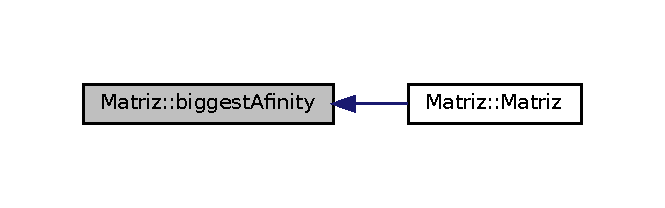
\includegraphics[width=319pt]{classMatriz_a2867d653d30b7fd8ca13e683bd7b8de6_icgraph}
\end{center}
\end{figure}
\mbox{\Hypertarget{classMatriz_a30e8aba7a2868aaa98f11d3037ff8319}\label{classMatriz_a30e8aba7a2868aaa98f11d3037ff8319}} 
\index{Matriz@{Matriz}!biggest\+Afinity\+Pair@{biggest\+Afinity\+Pair}}
\index{biggest\+Afinity\+Pair@{biggest\+Afinity\+Pair}!Matriz@{Matriz}}
\subsubsection{\texorpdfstring{biggest\+Afinity\+Pair()}{biggestAfinityPair()}}
{\footnotesize\ttfamily std\+::pair$<$ int, int $>$ Matriz\+::biggest\+Afinity\+Pair (\begin{DoxyParamCaption}{ }\end{DoxyParamCaption})}



returns a pair with the two nodes with the highest afinity 

\begin{DoxyReturn}{Returns}
std\+::pair$<$int,int$>$ 
\end{DoxyReturn}

\begin{DoxyCode}
58 \{
59   \textcolor{keywordtype}{float} biggestValue = 0;
60   std::vector<std::pair<int, int>> vectorAfinity;
61   \textcolor{keywordflow}{for} (\textcolor{keywordtype}{int} i = 0; i < matrix.size(); i++)
62   \{
63     \textcolor{keywordflow}{for} (\textcolor{keywordtype}{int} j = i + 1; j < matrix.size(); j++)
64     \{
65       \textcolor{keywordflow}{if} (matrix[i][j] >= biggestValue)
66       \{
67         biggestValue = matrix[i][j];
68       \}
69     \}
70   \}
71   \textcolor{keywordflow}{for} (\textcolor{keywordtype}{int} i = 0; i < matrix.size(); i++)
72   \{
73     \textcolor{keywordflow}{for} (\textcolor{keywordtype}{int} j = i + 1; j < matrix.size(); j++)
74     \{
75       \textcolor{keywordflow}{if} (matrix[i][j] == biggestValue)
76       \{
77         vectorAfinity.push\_back(std::pair<int, int>(i, j));
78       \}
79     \}
80   \}
81   \textcolor{keywordflow}{return} vectorAfinity[rand() % vectorAfinity.size()];
82 \}
\end{DoxyCode}
Here is the caller graph for this function\+:\nopagebreak
\begin{figure}[H]
\begin{center}
\leavevmode
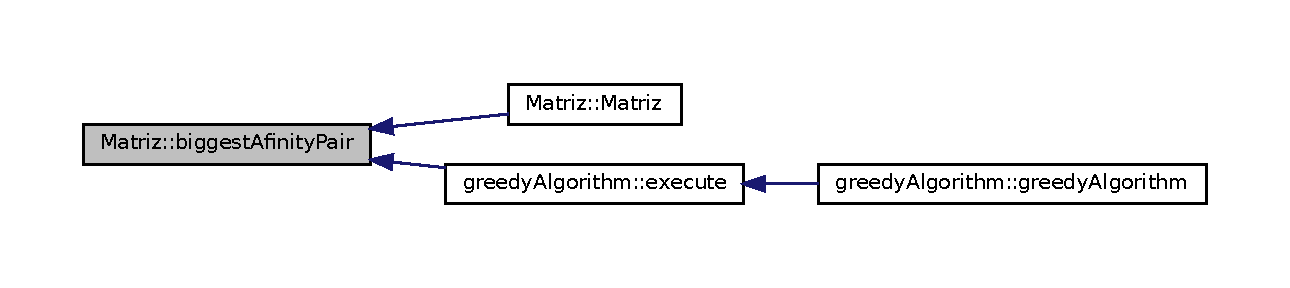
\includegraphics[width=350pt]{classMatriz_a30e8aba7a2868aaa98f11d3037ff8319_icgraph}
\end{center}
\end{figure}
\mbox{\Hypertarget{classMatriz_ad6915f9b31f93230a3ce05d01d23a47b}\label{classMatriz_ad6915f9b31f93230a3ce05d01d23a47b}} 
\index{Matriz@{Matriz}!get\+\_\+cols@{get\+\_\+cols}}
\index{get\+\_\+cols@{get\+\_\+cols}!Matriz@{Matriz}}
\subsubsection{\texorpdfstring{get\+\_\+cols()}{get\_cols()}}
{\footnotesize\ttfamily int Matriz\+::get\+\_\+cols (\begin{DoxyParamCaption}{ }\end{DoxyParamCaption})}



Get the cols object. 

\begin{DoxyReturn}{Returns}
int 
\end{DoxyReturn}

\begin{DoxyCode}
18 \{
19   \textcolor{keywordflow}{return} matrix[0].size();
20 \}
\end{DoxyCode}
Here is the caller graph for this function\+:\nopagebreak
\begin{figure}[H]
\begin{center}
\leavevmode
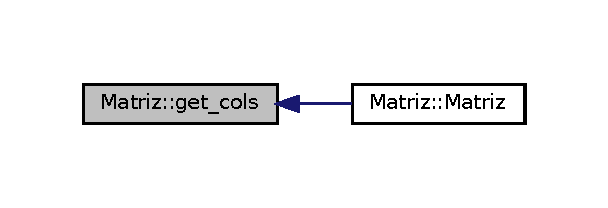
\includegraphics[width=292pt]{classMatriz_ad6915f9b31f93230a3ce05d01d23a47b_icgraph}
\end{center}
\end{figure}
\mbox{\Hypertarget{classMatriz_a1894d8447d3ae6992a43e46f93422b88}\label{classMatriz_a1894d8447d3ae6992a43e46f93422b88}} 
\index{Matriz@{Matriz}!get\+\_\+position@{get\+\_\+position}}
\index{get\+\_\+position@{get\+\_\+position}!Matriz@{Matriz}}
\subsubsection{\texorpdfstring{get\+\_\+position()}{get\_position()}}
{\footnotesize\ttfamily int Matriz\+::get\+\_\+position (\begin{DoxyParamCaption}\item[{int}]{row,  }\item[{int}]{col }\end{DoxyParamCaption})}



Get the position object. 


\begin{DoxyParams}{Parameters}
{\em row} & \\
\hline
{\em col} & \\
\hline
\end{DoxyParams}
\begin{DoxyReturn}{Returns}
int 
\end{DoxyReturn}

\begin{DoxyCode}
28 \{
29   \textcolor{keywordflow}{return} matrix[row][col];
30 \}
\end{DoxyCode}
Here is the caller graph for this function\+:\nopagebreak
\begin{figure}[H]
\begin{center}
\leavevmode
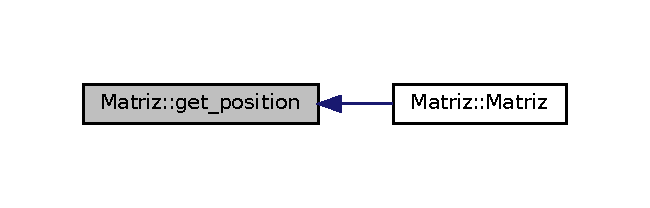
\includegraphics[width=312pt]{classMatriz_a1894d8447d3ae6992a43e46f93422b88_icgraph}
\end{center}
\end{figure}
\mbox{\Hypertarget{classMatriz_a6b18342f8c083baece693ff41185a206}\label{classMatriz_a6b18342f8c083baece693ff41185a206}} 
\index{Matriz@{Matriz}!get\+\_\+rows@{get\+\_\+rows}}
\index{get\+\_\+rows@{get\+\_\+rows}!Matriz@{Matriz}}
\subsubsection{\texorpdfstring{get\+\_\+rows()}{get\_rows()}}
{\footnotesize\ttfamily int Matriz\+::get\+\_\+rows (\begin{DoxyParamCaption}{ }\end{DoxyParamCaption})}



Get the rows object. 

\begin{DoxyReturn}{Returns}
int 
\end{DoxyReturn}

\begin{DoxyCode}
13 \{
14   \textcolor{keywordflow}{return} matrix.size();
15 \}
\end{DoxyCode}
Here is the caller graph for this function\+:\nopagebreak
\begin{figure}[H]
\begin{center}
\leavevmode
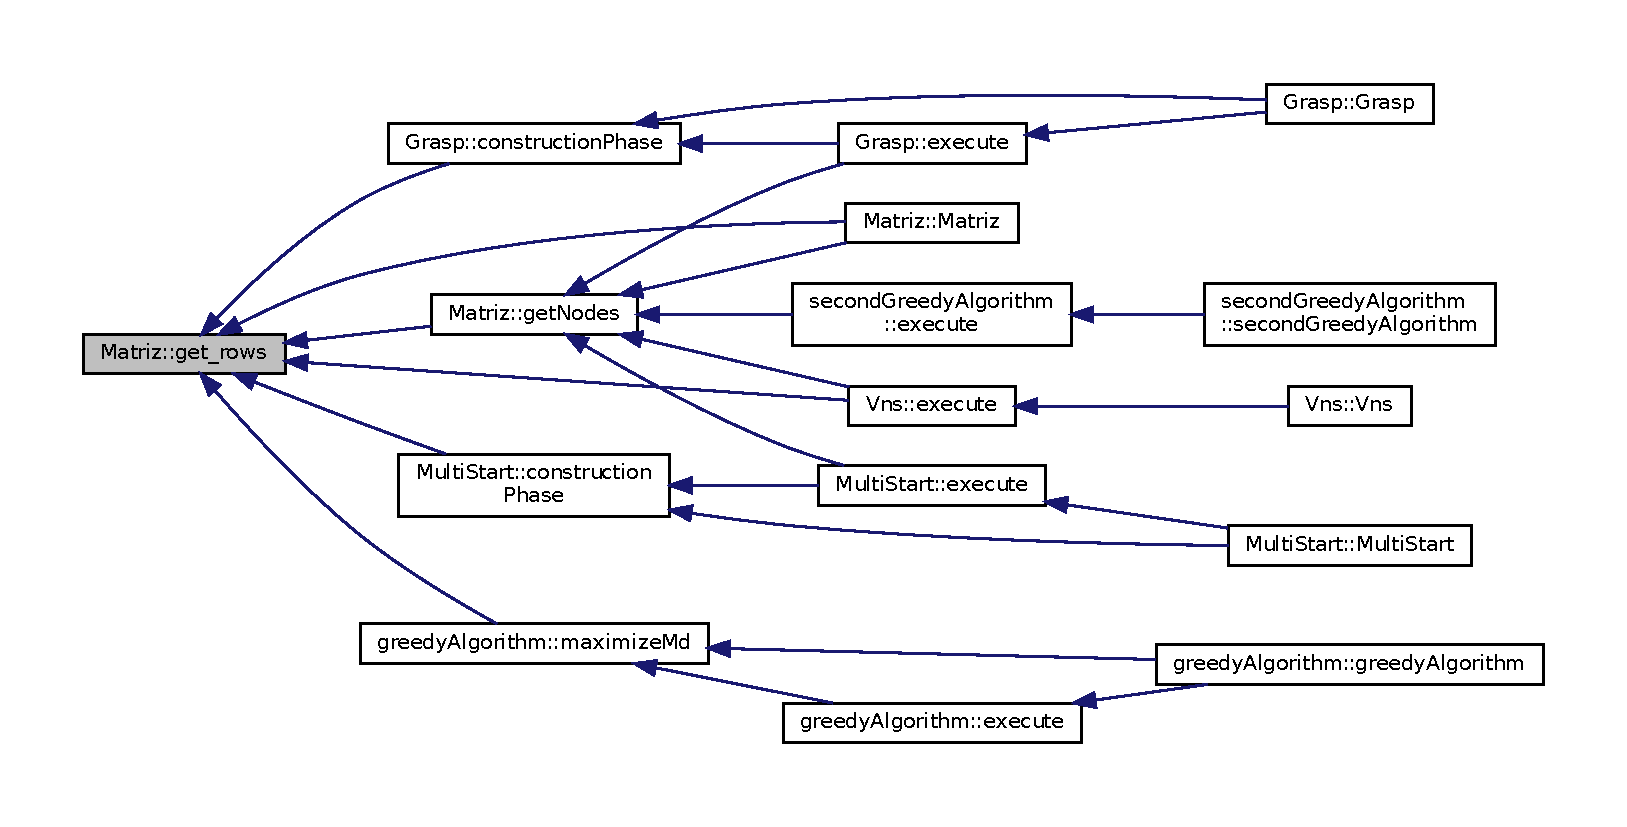
\includegraphics[width=350pt]{classMatriz_a6b18342f8c083baece693ff41185a206_icgraph}
\end{center}
\end{figure}
\mbox{\Hypertarget{classMatriz_a8df14a27d791f24206dd633b2a685c5b}\label{classMatriz_a8df14a27d791f24206dd633b2a685c5b}} 
\index{Matriz@{Matriz}!get\+Md@{get\+Md}}
\index{get\+Md@{get\+Md}!Matriz@{Matriz}}
\subsubsection{\texorpdfstring{get\+Md()}{getMd()}}
{\footnotesize\ttfamily float Matriz\+::get\+Md (\begin{DoxyParamCaption}\item[{std\+::vector$<$ int $>$}]{solution }\end{DoxyParamCaption})}



Returns the mean dispersion. 


\begin{DoxyParams}{Parameters}
{\em solution} & \\
\hline
\end{DoxyParams}
\begin{DoxyReturn}{Returns}
float 
\end{DoxyReturn}

\begin{DoxyCode}
85 \{
86   \textcolor{keywordtype}{float} sumOfAfinities = 0;
87   \textcolor{keywordflow}{for} (\textcolor{keywordtype}{int} i = 0; i < solution.size(); i++)
88   \{
89     \textcolor{keywordflow}{for} (\textcolor{keywordtype}{int} j = i + 1; j < solution.size(); j++)
90     \{
91       sumOfAfinities += matrix[solution[i]][solution[j]];
92     \}
93   \}
94   \textcolor{keywordflow}{return} sumOfAfinities / solution.size();
95 \}
\end{DoxyCode}
Here is the caller graph for this function\+:
\nopagebreak
\begin{figure}[H]
\begin{center}
\leavevmode
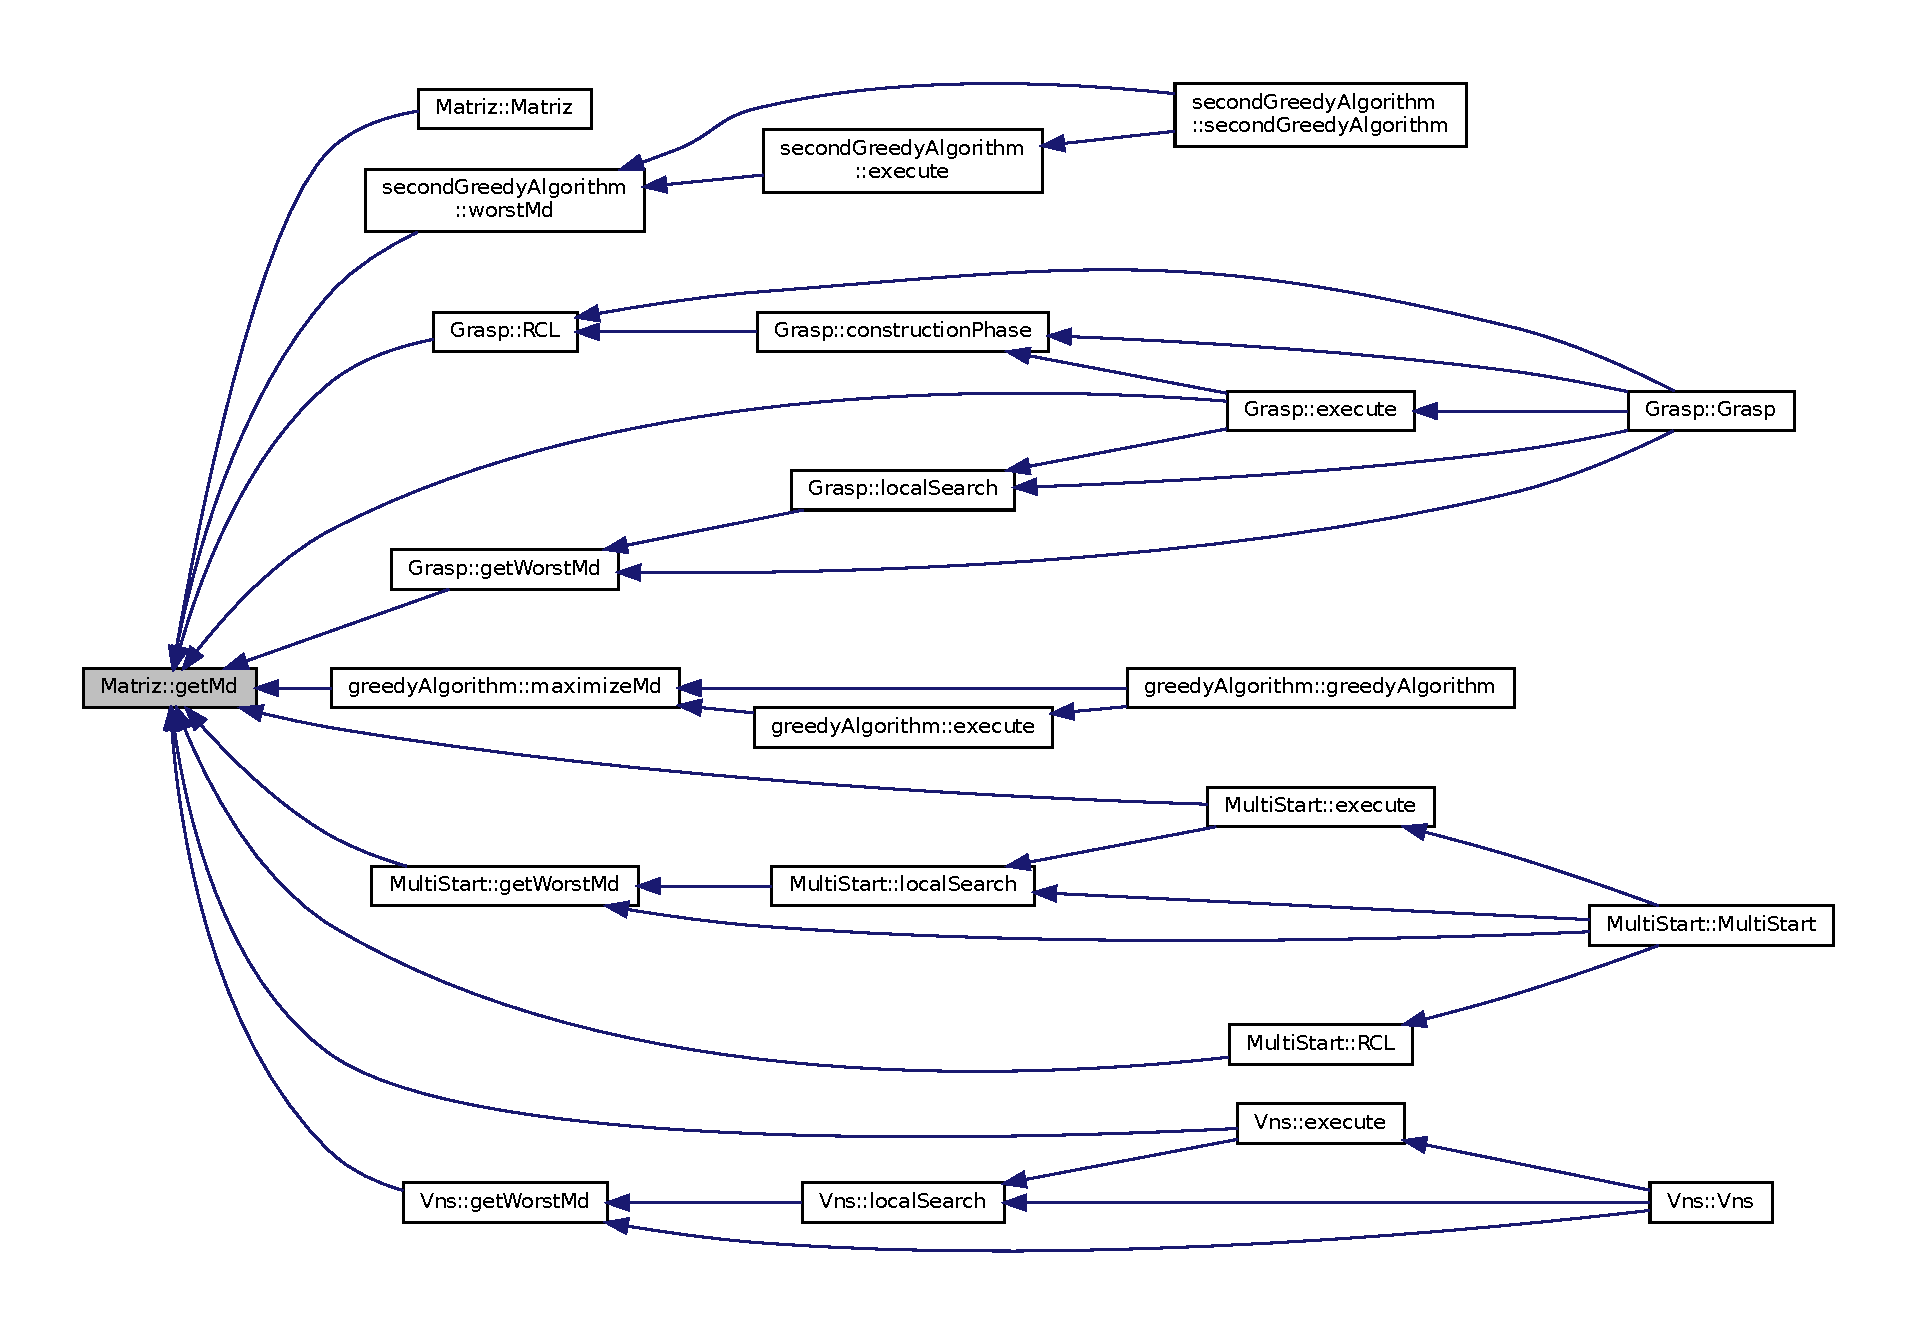
\includegraphics[width=350pt]{classMatriz_a8df14a27d791f24206dd633b2a685c5b_icgraph}
\end{center}
\end{figure}
\mbox{\Hypertarget{classMatriz_a61efbcc7ea661059ed0dfad32b5273cf}\label{classMatriz_a61efbcc7ea661059ed0dfad32b5273cf}} 
\index{Matriz@{Matriz}!get\+Md\+Pair@{get\+Md\+Pair}}
\index{get\+Md\+Pair@{get\+Md\+Pair}!Matriz@{Matriz}}
\subsubsection{\texorpdfstring{get\+Md\+Pair()}{getMdPair()}}
{\footnotesize\ttfamily float Matriz\+::get\+Md\+Pair (\begin{DoxyParamCaption}\item[{std\+::vector$<$ std\+::pair$<$ int, int $>$$>$}]{solution }\end{DoxyParamCaption})}



Returns the mean dispersion. 


\begin{DoxyParams}{Parameters}
{\em solution} & \\
\hline
\end{DoxyParams}
\begin{DoxyReturn}{Returns}
float 
\end{DoxyReturn}

\begin{DoxyCode}
126 \{
127   \textcolor{keywordtype}{float} sumOfAfinities = 0;
128   \textcolor{keywordflow}{for} (\textcolor{keywordtype}{int} i = 0; i < solution.size(); i++)
129   \{
130       sumOfAfinities += matrix[solution[i].first][solution[i].second];
131   \}
132   \textcolor{keywordflow}{return} sumOfAfinities / solution.size();
133 \}
\end{DoxyCode}
Here is the caller graph for this function\+:
\nopagebreak
\begin{figure}[H]
\begin{center}
\leavevmode
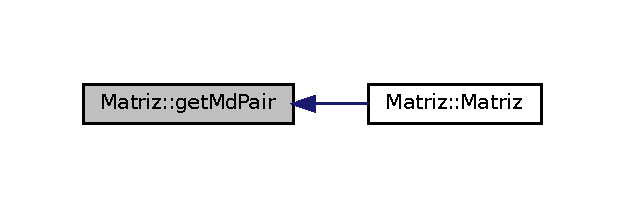
\includegraphics[width=300pt]{classMatriz_a61efbcc7ea661059ed0dfad32b5273cf_icgraph}
\end{center}
\end{figure}
\mbox{\Hypertarget{classMatriz_a394b84a5ec13fd2f4d202ab218680afe}\label{classMatriz_a394b84a5ec13fd2f4d202ab218680afe}} 
\index{Matriz@{Matriz}!get\+Nodes@{get\+Nodes}}
\index{get\+Nodes@{get\+Nodes}!Matriz@{Matriz}}
\subsubsection{\texorpdfstring{get\+Nodes()}{getNodes()}}
{\footnotesize\ttfamily std\+::vector$<$ int $>$ Matriz\+::get\+Nodes (\begin{DoxyParamCaption}{ }\end{DoxyParamCaption})}



Returns a vector with all the nodes. 

\begin{DoxyReturn}{Returns}
std\+::vector$<$int$>$ 
\end{DoxyReturn}

\begin{DoxyCode}
135                                 \{
136   std::vector<int> result;
137   \textcolor{keywordflow}{for}(\textcolor{keywordtype}{int} i = 0; i < this->\hyperlink{classMatriz_a6b18342f8c083baece693ff41185a206}{get\_rows}(); i++) \{
138     result.push\_back(i);
139   \}
140   \textcolor{keywordflow}{return} result;
141 \}
\end{DoxyCode}
Here is the call graph for this function\+:
\nopagebreak
\begin{figure}[H]
\begin{center}
\leavevmode
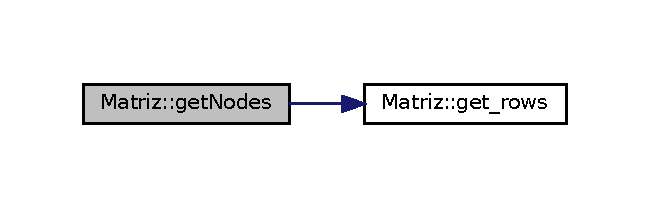
\includegraphics[width=312pt]{classMatriz_a394b84a5ec13fd2f4d202ab218680afe_cgraph}
\end{center}
\end{figure}
Here is the caller graph for this function\+:
\nopagebreak
\begin{figure}[H]
\begin{center}
\leavevmode
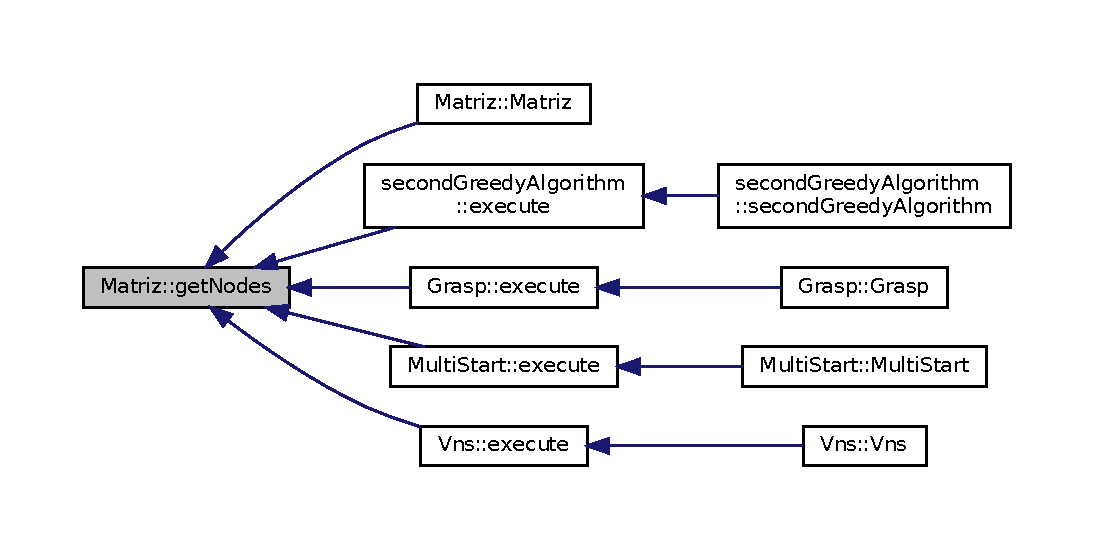
\includegraphics[width=350pt]{classMatriz_a394b84a5ec13fd2f4d202ab218680afe_icgraph}
\end{center}
\end{figure}
\mbox{\Hypertarget{classMatriz_ad2adc857ff1738ebfb7fe42de408737b}\label{classMatriz_ad2adc857ff1738ebfb7fe42de408737b}} 
\index{Matriz@{Matriz}!operator\mbox{[}\mbox{]}@{operator[]}}
\index{operator\mbox{[}\mbox{]}@{operator[]}!Matriz@{Matriz}}
\subsubsection{\texorpdfstring{operator[]()}{operator[]()}}
{\footnotesize\ttfamily std\+::vector$<$ int $>$ \& Matriz\+::operator\mbox{[}$\,$\mbox{]} (\begin{DoxyParamCaption}\item[{int}]{index }\end{DoxyParamCaption})}



Operator \mbox{[}\mbox{]} overload. 


\begin{DoxyParams}{Parameters}
{\em index} & \\
\hline
\end{DoxyParams}
\begin{DoxyReturn}{Returns}
std\+::vector$<$int$>$\& 
\end{DoxyReturn}

\begin{DoxyCode}
45 \{
46   \textcolor{keywordflow}{if} (index >= matrix.size())
47   \{
48     std::cerr << \textcolor{stringliteral}{"Index fuera de rango"} << std::endl;
49     std::exit(0);
50   \}
51   \textcolor{keywordflow}{else}
52   \{
53     \textcolor{keywordflow}{return} matrix[index];
54   \}
55 \}
\end{DoxyCode}
Here is the caller graph for this function\+:
\nopagebreak
\begin{figure}[H]
\begin{center}
\leavevmode
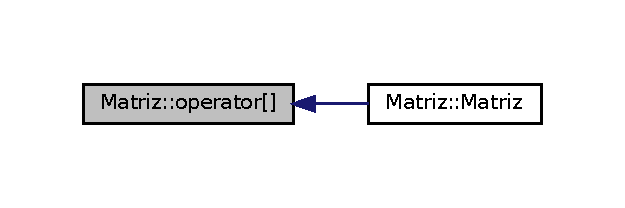
\includegraphics[width=300pt]{classMatriz_ad2adc857ff1738ebfb7fe42de408737b_icgraph}
\end{center}
\end{figure}
\mbox{\Hypertarget{classMatriz_aa929f933e9088dc0efecaa9a46d555d9}\label{classMatriz_aa929f933e9088dc0efecaa9a46d555d9}} 
\index{Matriz@{Matriz}!resize\+Matrix@{resize\+Matrix}}
\index{resize\+Matrix@{resize\+Matrix}!Matriz@{Matriz}}
\subsubsection{\texorpdfstring{resize\+Matrix()}{resizeMatrix()}}
{\footnotesize\ttfamily void Matriz\+::resize\+Matrix (\begin{DoxyParamCaption}\item[{int}]{rows,  }\item[{int}]{cols }\end{DoxyParamCaption})}



Change the matrix\textquotesingle{}s dimensions. 


\begin{DoxyParams}{Parameters}
{\em rows} & \\
\hline
{\em cols} & \\
\hline
\end{DoxyParams}

\begin{DoxyCode}
4 \{
5   \textcolor{keywordflow}{for} (\textcolor{keywordtype}{int} i = 0; i < matrix.size(); i++)
6   \{
7     matrix[i].resize(cols);
8   \}
9   matrix.resize(rows, std::vector<int>(cols));
10 \}
\end{DoxyCode}
Here is the caller graph for this function\+:
\nopagebreak
\begin{figure}[H]
\begin{center}
\leavevmode
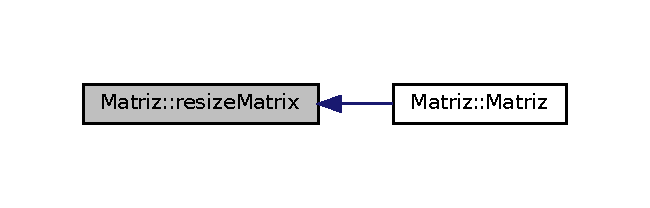
\includegraphics[width=312pt]{classMatriz_aa929f933e9088dc0efecaa9a46d555d9_icgraph}
\end{center}
\end{figure}
\mbox{\Hypertarget{classMatriz_a71fea2383ce785254c2f27da25ef70c8}\label{classMatriz_a71fea2383ce785254c2f27da25ef70c8}} 
\index{Matriz@{Matriz}!set\+\_\+position@{set\+\_\+position}}
\index{set\+\_\+position@{set\+\_\+position}!Matriz@{Matriz}}
\subsubsection{\texorpdfstring{set\+\_\+position()}{set\_position()}}
{\footnotesize\ttfamily void Matriz\+::set\+\_\+position (\begin{DoxyParamCaption}\item[{int}]{row,  }\item[{int}]{col,  }\item[{int}]{value }\end{DoxyParamCaption})}



Set the position object. 


\begin{DoxyParams}{Parameters}
{\em row} & \\
\hline
{\em col} & \\
\hline
{\em value} & \\
\hline
\end{DoxyParams}

\begin{DoxyCode}
23 \{
24   matrix[row][col] = value;
25 \}
\end{DoxyCode}
Here is the caller graph for this function\+:
\nopagebreak
\begin{figure}[H]
\begin{center}
\leavevmode
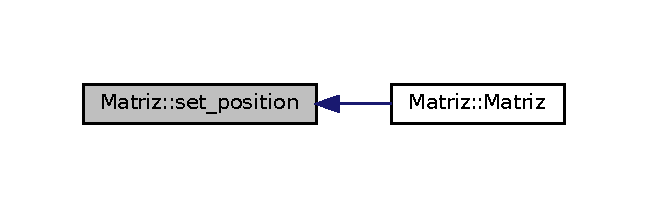
\includegraphics[width=311pt]{classMatriz_a71fea2383ce785254c2f27da25ef70c8_icgraph}
\end{center}
\end{figure}


The documentation for this class was generated from the following files\+:\begin{DoxyCompactItemize}
\item 
include/\hyperlink{matrix_8hpp}{matrix.\+hpp}\item 
src/matrix.\+cpp\end{DoxyCompactItemize}

\hypertarget{classMultiStart}{}\section{Multi\+Start Class Reference}
\label{classMultiStart}\index{Multi\+Start@{Multi\+Start}}


\hyperlink{classMultiStart}{Multi\+Start} implementation to solve Max Mean.  




{\ttfamily \#include $<$multi\+Start.\+hpp$>$}



Inheritance diagram for Multi\+Start\+:\nopagebreak
\begin{figure}[H]
\begin{center}
\leavevmode
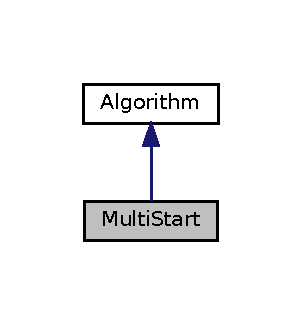
\includegraphics[width=145pt]{classMultiStart__inherit__graph}
\end{center}
\end{figure}


Collaboration diagram for Multi\+Start\+:\nopagebreak
\begin{figure}[H]
\begin{center}
\leavevmode
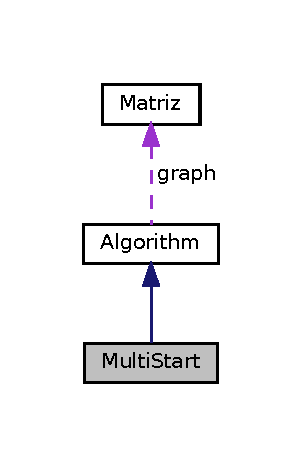
\includegraphics[width=145pt]{classMultiStart__coll__graph}
\end{center}
\end{figure}
\subsection*{Public Member Functions}
\begin{DoxyCompactItemize}
\item 
\hyperlink{classMultiStart_ae16c330042c4b1dfb87dae8312d07a65}{Multi\+Start} (std\+::string filename, int iter, int noimprov, bool anx)
\begin{DoxyCompactList}\small\item\em Construct a new Multi Start object. \end{DoxyCompactList}\item 
std\+::vector$<$ int $>$ \hyperlink{classMultiStart_a29c5796648ede3e6c7fe8ca8043f8187}{construction\+Phase} (std\+::vector$<$ int $>$ first\+Candidates)
\begin{DoxyCompactList}\small\item\em Function to create a initial solution for the problem. \end{DoxyCompactList}\item 
std\+::vector$<$ int $>$ \hyperlink{classMultiStart_a456dc441b6e7028aa86a0488830f9bc1}{R\+CL} (std\+::vector$<$ int $>$, std\+::vector$<$ int $>$)
\begin{DoxyCompactList}\small\item\em Function to create a R\+CL array based on an initial solution. \end{DoxyCompactList}\item 
std\+::vector$<$ int $>$ \hyperlink{classMultiStart_af27ae5dbba5f924070f103b7bf5987a3}{local\+Search} (std\+::vector$<$ int $>$, std\+::vector$<$ int $>$)
\begin{DoxyCompactList}\small\item\em Function that uses a greedy algorithm to improve the solution. \end{DoxyCompactList}\item 
std\+::pair$<$ int, bool $>$ \hyperlink{classMultiStart_a0ad5ed40a5c4ab964cb27f79343eed98}{get\+Worst\+Md} (std\+::vector$<$ int $>$)
\begin{DoxyCompactList}\small\item\em Return the worst node (worst afinity) in the actual solution. \end{DoxyCompactList}\item 
std\+::vector$<$ int $>$ \hyperlink{classMultiStart_a9d842b1f602c4b8a47bf6d88d483ccae}{execute} ()
\begin{DoxyCompactList}\small\item\em Method that executes the algorithm. \end{DoxyCompactList}\end{DoxyCompactItemize}
\subsection*{Additional Inherited Members}


\subsection{Detailed Description}
\hyperlink{classMultiStart}{Multi\+Start} implementation to solve Max Mean. 

\subsection{Constructor \& Destructor Documentation}
\mbox{\Hypertarget{classMultiStart_ae16c330042c4b1dfb87dae8312d07a65}\label{classMultiStart_ae16c330042c4b1dfb87dae8312d07a65}} 
\index{Multi\+Start@{Multi\+Start}!Multi\+Start@{Multi\+Start}}
\index{Multi\+Start@{Multi\+Start}!Multi\+Start@{Multi\+Start}}
\subsubsection{\texorpdfstring{Multi\+Start()}{MultiStart()}}
{\footnotesize\ttfamily Multi\+Start\+::\+Multi\+Start (\begin{DoxyParamCaption}\item[{std\+::string}]{filename,  }\item[{int}]{iter,  }\item[{int}]{noimprov,  }\item[{bool}]{anx }\end{DoxyParamCaption})\hspace{0.3cm}{\ttfamily [inline]}}



Construct a new Multi Start object. 


\begin{DoxyParams}{Parameters}
{\em filename} & \\
\hline
{\em iter} & \\
\hline
{\em noimprov} & \\
\hline
{\em anx} & \\
\hline
\end{DoxyParams}

\begin{DoxyCode}
37 : \hyperlink{classAlgorithm_a89df1d2c6751f70733f38daa0ee2a13b}{Algorithm}(filename), Iterations(iter), NoImprov(noimprov), anxious(anx) \{\}
\end{DoxyCode}
Here is the call graph for this function\+:\nopagebreak
\begin{figure}[H]
\begin{center}
\leavevmode
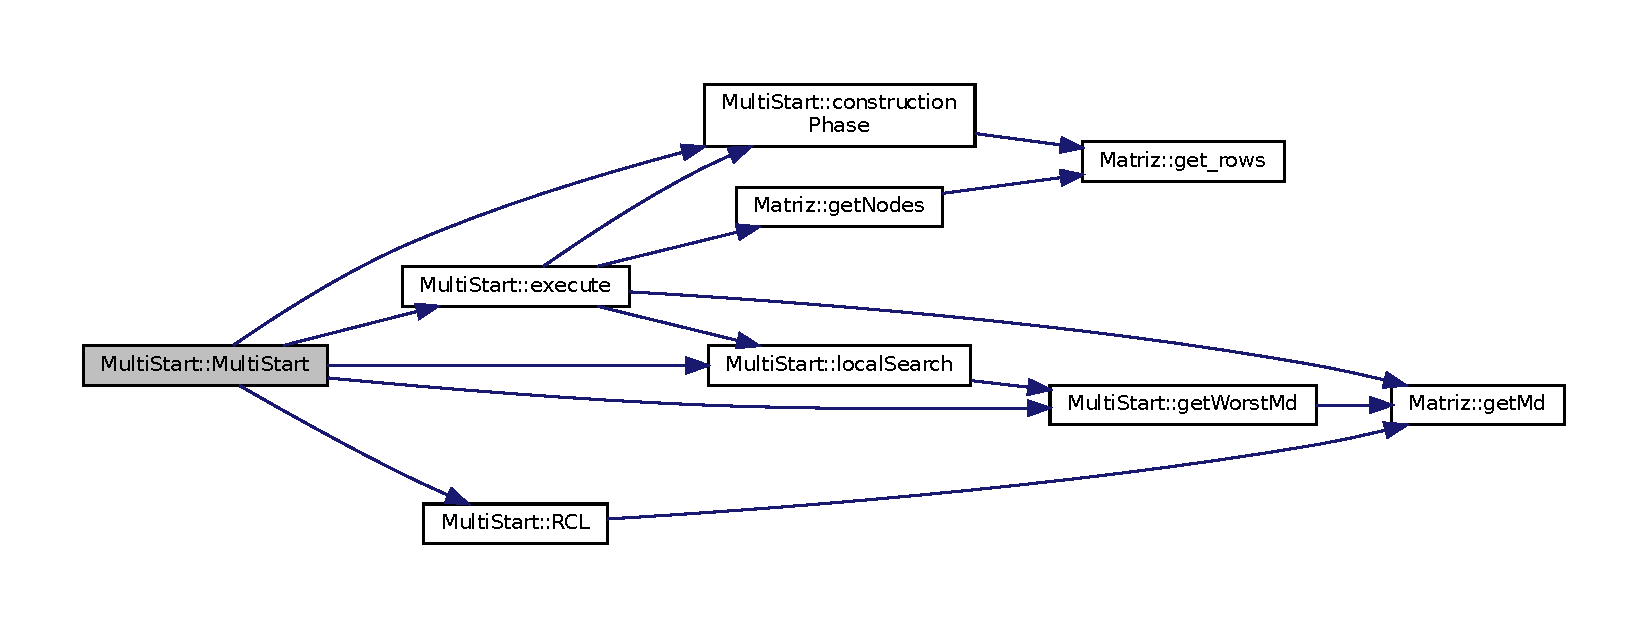
\includegraphics[width=350pt]{classMultiStart_ae16c330042c4b1dfb87dae8312d07a65_cgraph}
\end{center}
\end{figure}


\subsection{Member Function Documentation}
\mbox{\Hypertarget{classMultiStart_a29c5796648ede3e6c7fe8ca8043f8187}\label{classMultiStart_a29c5796648ede3e6c7fe8ca8043f8187}} 
\index{Multi\+Start@{Multi\+Start}!construction\+Phase@{construction\+Phase}}
\index{construction\+Phase@{construction\+Phase}!Multi\+Start@{Multi\+Start}}
\subsubsection{\texorpdfstring{construction\+Phase()}{constructionPhase()}}
{\footnotesize\ttfamily std\+::vector$<$ int $>$ Multi\+Start\+::construction\+Phase (\begin{DoxyParamCaption}\item[{std\+::vector$<$ int $>$}]{first\+Candidates }\end{DoxyParamCaption})}



Function to create a initial solution for the problem. 


\begin{DoxyParams}{Parameters}
{\em first\+Candidates} & \\
\hline
\end{DoxyParams}
\begin{DoxyReturn}{Returns}
std\+::vector$<$int$>$ 
\end{DoxyReturn}

\begin{DoxyCode}
4 \{
5   std::vector<int> solution;
6   \textcolor{keywordtype}{int} firstNode = rand() % firstCandidates.size();
7   solution.push\_back(firstCandidates[firstNode]);
8   \textcolor{keywordtype}{int} solutionSize = (rand() % (graph.\hyperlink{classMatriz_a6b18342f8c083baece693ff41185a206}{get\_rows}() - 2)) + 2;
9   \textcolor{keywordflow}{while} (solution.size() < solutionSize)
10   \{
11     \textcolor{keywordtype}{int} randomSelection = rand() % firstCandidates.size();
12     \textcolor{keywordflow}{if} (std::find(solution.begin(), solution.end(), firstCandidates[randomSelection]) == solution.end())
13     \{
14       solution.push\_back(randomSelection);
15     \}
16   \}
17   \textcolor{keywordflow}{return} solution;
18 \}
\end{DoxyCode}
Here is the call graph for this function\+:\nopagebreak
\begin{figure}[H]
\begin{center}
\leavevmode
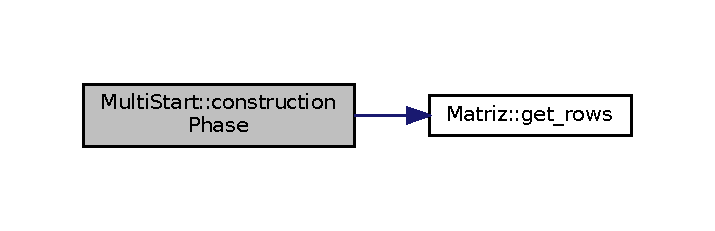
\includegraphics[width=343pt]{classMultiStart_a29c5796648ede3e6c7fe8ca8043f8187_cgraph}
\end{center}
\end{figure}
Here is the caller graph for this function\+:\nopagebreak
\begin{figure}[H]
\begin{center}
\leavevmode
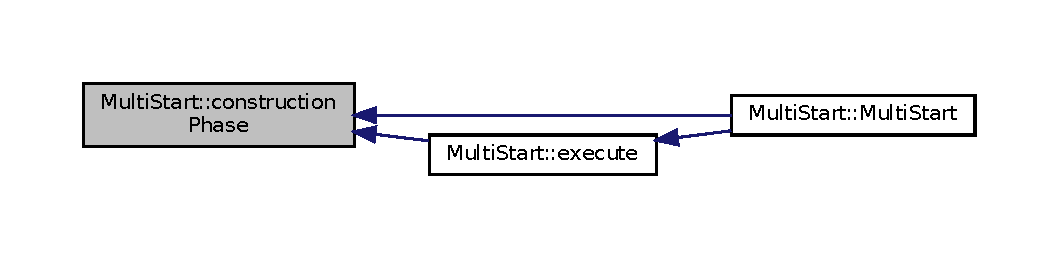
\includegraphics[width=350pt]{classMultiStart_a29c5796648ede3e6c7fe8ca8043f8187_icgraph}
\end{center}
\end{figure}
\mbox{\Hypertarget{classMultiStart_a9d842b1f602c4b8a47bf6d88d483ccae}\label{classMultiStart_a9d842b1f602c4b8a47bf6d88d483ccae}} 
\index{Multi\+Start@{Multi\+Start}!execute@{execute}}
\index{execute@{execute}!Multi\+Start@{Multi\+Start}}
\subsubsection{\texorpdfstring{execute()}{execute()}}
{\footnotesize\ttfamily std\+::vector$<$ int $>$ Multi\+Start\+::execute (\begin{DoxyParamCaption}{ }\end{DoxyParamCaption})\hspace{0.3cm}{\ttfamily [virtual]}}



Method that executes the algorithm. 

\begin{DoxyReturn}{Returns}
std\+::vector$<$int$>$ 
\end{DoxyReturn}


Implements \hyperlink{classAlgorithm_af6ea9eb9a6dbd41896e3fd7dabac096b}{Algorithm}.


\begin{DoxyCode}
99 \{
100   std::vector<int> firstNodes = graph.\hyperlink{classMatriz_a394b84a5ec13fd2f4d202ab218680afe}{getNodes}();
101   std::vector<int> bestSolution;
102   bestSolution.push\_back(0);
103   \textcolor{keywordtype}{float} bestDistance = graph.\hyperlink{classMatriz_a8df14a27d791f24206dd633b2a685c5b}{getMd}(bestSolution);
104   \textcolor{keywordtype}{int} iterations = 0;
105   \textcolor{keywordtype}{int} noImprovement = 0;
106   \textcolor{keywordflow}{while} (iterations < this->Iterations && noImprovement < this->NoImprov)
107   \{
108     iterations++;
109     std::vector<int> initialSol = \hyperlink{classMultiStart_a29c5796648ede3e6c7fe8ca8043f8187}{constructionPhase}(firstNodes);
110     std::vector<int> localSearchVector = \hyperlink{classMultiStart_af27ae5dbba5f924070f103b7bf5987a3}{localSearch}(initialSol, firstNodes);
111     \textcolor{keywordtype}{float} testMd = graph.\hyperlink{classMatriz_a8df14a27d791f24206dd633b2a685c5b}{getMd}(localSearchVector);
112     \textcolor{keywordflow}{if} (testMd > bestDistance)
113     \{
114       bestSolution = localSearchVector;
115       bestDistance = testMd;
116       noImprovement = 0;
117     \}
118     \textcolor{keywordflow}{else}
119     \{
120       noImprovement++;
121     \}
122   \}
123 
124   \textcolor{keywordflow}{return} bestSolution;
125 \}
\end{DoxyCode}
Here is the call graph for this function\+:\nopagebreak
\begin{figure}[H]
\begin{center}
\leavevmode
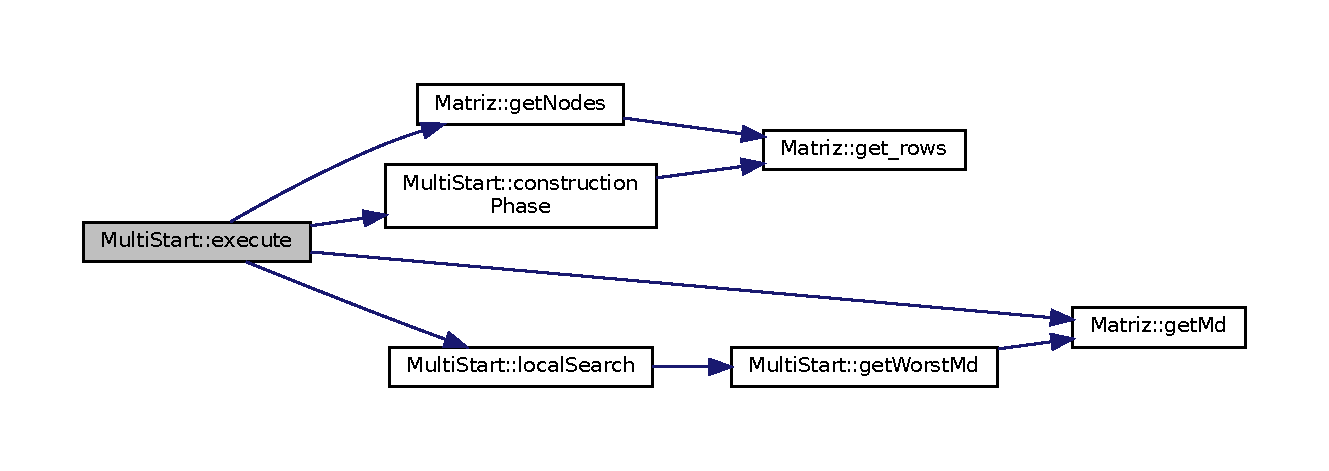
\includegraphics[width=350pt]{classMultiStart_a9d842b1f602c4b8a47bf6d88d483ccae_cgraph}
\end{center}
\end{figure}
Here is the caller graph for this function\+:\nopagebreak
\begin{figure}[H]
\begin{center}
\leavevmode
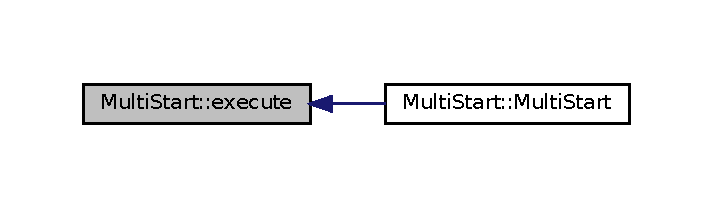
\includegraphics[width=342pt]{classMultiStart_a9d842b1f602c4b8a47bf6d88d483ccae_icgraph}
\end{center}
\end{figure}
\mbox{\Hypertarget{classMultiStart_a0ad5ed40a5c4ab964cb27f79343eed98}\label{classMultiStart_a0ad5ed40a5c4ab964cb27f79343eed98}} 
\index{Multi\+Start@{Multi\+Start}!get\+Worst\+Md@{get\+Worst\+Md}}
\index{get\+Worst\+Md@{get\+Worst\+Md}!Multi\+Start@{Multi\+Start}}
\subsubsection{\texorpdfstring{get\+Worst\+Md()}{getWorstMd()}}
{\footnotesize\ttfamily std\+::pair$<$ int, bool $>$ Multi\+Start\+::get\+Worst\+Md (\begin{DoxyParamCaption}\item[{std\+::vector$<$ int $>$}]{solution }\end{DoxyParamCaption})}



Return the worst node (worst afinity) in the actual solution. 

\begin{DoxyReturn}{Returns}
std\+::pair$<$int,bool$>$ 
\end{DoxyReturn}

\begin{DoxyCode}
67 \{
68   std::vector<std::pair<int, bool>> vertexVector;
69   std::pair<int, bool> vertex(-1, \textcolor{keyword}{false});
70   vertexVector.push\_back(vertex);
71   \textcolor{keywordtype}{float} currentDistance = graph.\hyperlink{classMatriz_a8df14a27d791f24206dd633b2a685c5b}{getMd}(solution);
72   \textcolor{keywordtype}{float} currentEdgeSum = currentDistance * solution.size();
73   \textcolor{keywordflow}{for} (\textcolor{keywordtype}{int} i = 0; i < solution.size(); i++)
74   \{
75     \textcolor{keywordtype}{int} vertex = solution[i];
76     solution.erase(solution.begin() + i);
77     \textcolor{keywordtype}{float} nextMd = graph.\hyperlink{classMatriz_a8df14a27d791f24206dd633b2a685c5b}{getMd}(solution);
78     solution.insert(solution.begin() + i, vertex);
79     \textcolor{keywordflow}{if} (nextMd > currentDistance)
80     \{
81       \textcolor{keywordflow}{if} (anxious)
82       \{
83         \textcolor{keywordflow}{return} std::pair<int, bool>(i, \textcolor{keyword}{true});
84         ;
85       \}
86       currentDistance = nextMd;
87       vertexVector.clear();
88       vertexVector.push\_back(std::pair<int, bool>(i, \textcolor{keyword}{true}));
89     \}
90     \textcolor{keywordflow}{else} \textcolor{keywordflow}{if} (nextMd == currentDistance)
91     \{
92       vertexVector.push\_back(std::pair<int, bool>(i, \textcolor{keyword}{true}));
93     \}
94   \}
95   \textcolor{keywordflow}{return} vertexVector[rand() % vertexVector.size()];
96 \}
\end{DoxyCode}
Here is the call graph for this function\+:\nopagebreak
\begin{figure}[H]
\begin{center}
\leavevmode
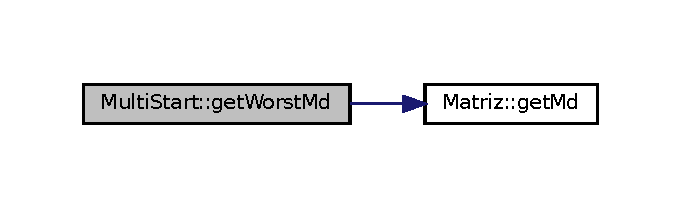
\includegraphics[width=327pt]{classMultiStart_a0ad5ed40a5c4ab964cb27f79343eed98_cgraph}
\end{center}
\end{figure}
Here is the caller graph for this function\+:\nopagebreak
\begin{figure}[H]
\begin{center}
\leavevmode
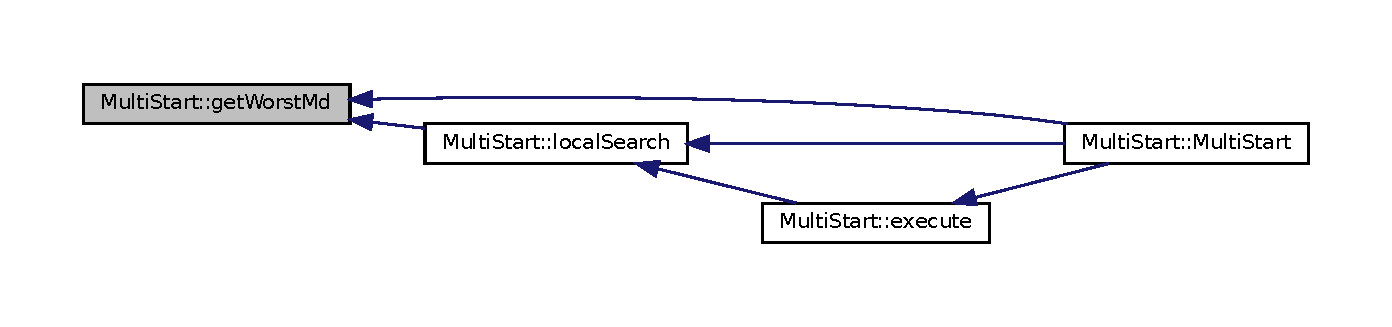
\includegraphics[width=350pt]{classMultiStart_a0ad5ed40a5c4ab964cb27f79343eed98_icgraph}
\end{center}
\end{figure}
\mbox{\Hypertarget{classMultiStart_af27ae5dbba5f924070f103b7bf5987a3}\label{classMultiStart_af27ae5dbba5f924070f103b7bf5987a3}} 
\index{Multi\+Start@{Multi\+Start}!local\+Search@{local\+Search}}
\index{local\+Search@{local\+Search}!Multi\+Start@{Multi\+Start}}
\subsubsection{\texorpdfstring{local\+Search()}{localSearch()}}
{\footnotesize\ttfamily std\+::vector$<$ int $>$ Multi\+Start\+::local\+Search (\begin{DoxyParamCaption}\item[{std\+::vector$<$ int $>$}]{solution,  }\item[{std\+::vector$<$ int $>$}]{first\+Candidates }\end{DoxyParamCaption})}



Function that uses a greedy algorithm to improve the solution. 

\begin{DoxyReturn}{Returns}
std\+::vector$<$int$>$ 
\end{DoxyReturn}

\begin{DoxyCode}
51 \{
52   \textcolor{keywordtype}{bool} improvement = \textcolor{keyword}{true};
53   \textcolor{keywordflow}{while} (improvement)
54   \{
55     improvement = \textcolor{keyword}{false};
56     std::pair<int, bool> worst = \hyperlink{classMultiStart_a0ad5ed40a5c4ab964cb27f79343eed98}{getWorstMd}(solution);
57     \textcolor{keywordflow}{if} (worst.second)
58     \{
59       improvement = \textcolor{keyword}{true};
60       solution.erase(solution.begin() + worst.first);
61     \}
62   \}
63   \textcolor{keywordflow}{return} solution;
64 \}
\end{DoxyCode}
Here is the call graph for this function\+:\nopagebreak
\begin{figure}[H]
\begin{center}
\leavevmode
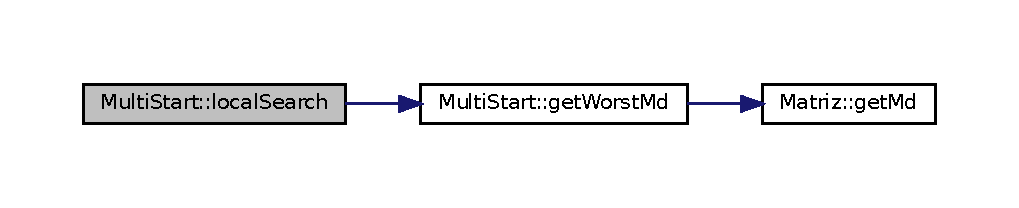
\includegraphics[width=350pt]{classMultiStart_af27ae5dbba5f924070f103b7bf5987a3_cgraph}
\end{center}
\end{figure}
Here is the caller graph for this function\+:\nopagebreak
\begin{figure}[H]
\begin{center}
\leavevmode
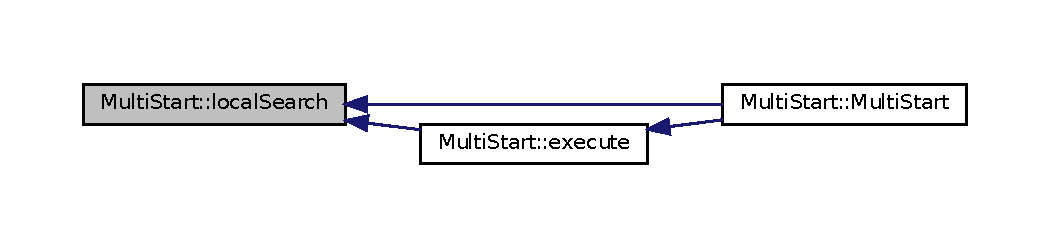
\includegraphics[width=350pt]{classMultiStart_af27ae5dbba5f924070f103b7bf5987a3_icgraph}
\end{center}
\end{figure}
\mbox{\Hypertarget{classMultiStart_a456dc441b6e7028aa86a0488830f9bc1}\label{classMultiStart_a456dc441b6e7028aa86a0488830f9bc1}} 
\index{Multi\+Start@{Multi\+Start}!R\+CL@{R\+CL}}
\index{R\+CL@{R\+CL}!Multi\+Start@{Multi\+Start}}
\subsubsection{\texorpdfstring{R\+C\+L()}{RCL()}}
{\footnotesize\ttfamily std\+::vector$<$ int $>$ Multi\+Start\+::\+R\+CL (\begin{DoxyParamCaption}\item[{std\+::vector$<$ int $>$}]{solution,  }\item[{std\+::vector$<$ int $>$}]{first\+Candidates }\end{DoxyParamCaption})}



Function to create a R\+CL array based on an initial solution. 

\begin{DoxyReturn}{Returns}
std\+::vector$<$int$>$ 
\end{DoxyReturn}

\begin{DoxyCode}
21 \{
22   std::vector<int> sortedNodes;
23   std::vector<float> sortedDistances;
24   std::vector<int> rclVector;
25   \textcolor{keywordflow}{for} (\textcolor{keywordtype}{int} i = 0; i < firstCandidates.size(); i++)
26   \{
27     \textcolor{keywordflow}{if} (std::find(solution.begin(), solution.end(), firstCandidates[i]) == solution.end())
28     \{
29       solution.push\_back(firstCandidates[i]);
30       \textcolor{keywordtype}{float} testMd = graph.\hyperlink{classMatriz_a8df14a27d791f24206dd633b2a685c5b}{getMd}(solution);
31       solution.pop\_back();
32       \textcolor{keywordtype}{int} position = 0;
33       \textcolor{keywordflow}{for} (\textcolor{keywordtype}{int} j = 0; j < sortedDistances.size(); j++)
34       \{
35         \textcolor{keywordflow}{if} (testMd < sortedDistances[j])
36         \{
37           position++;
38         \}
39       \}
40       sortedDistances.insert(sortedDistances.begin() + position, testMd);
41       sortedNodes.insert(sortedNodes.begin() + position, firstCandidates[i]);
42     \}
43   \}
44   \textcolor{keywordtype}{int} percent = (sortedNodes.size() / (1 / 0.2));
45   percent = percent == 0 ? 1 : percent;
46   std::copy(sortedNodes.begin(), sortedNodes.begin() + percent, std::back\_inserter(rclVector));
47   \textcolor{keywordflow}{return} rclVector;
48 \}
\end{DoxyCode}
Here is the call graph for this function\+:\nopagebreak
\begin{figure}[H]
\begin{center}
\leavevmode
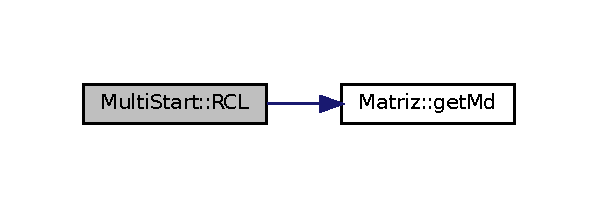
\includegraphics[width=287pt]{classMultiStart_a456dc441b6e7028aa86a0488830f9bc1_cgraph}
\end{center}
\end{figure}
Here is the caller graph for this function\+:\nopagebreak
\begin{figure}[H]
\begin{center}
\leavevmode
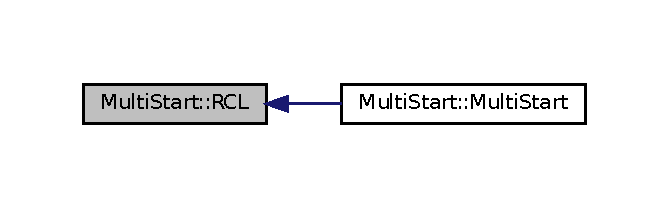
\includegraphics[width=321pt]{classMultiStart_a456dc441b6e7028aa86a0488830f9bc1_icgraph}
\end{center}
\end{figure}


The documentation for this class was generated from the following files\+:\begin{DoxyCompactItemize}
\item 
include/\hyperlink{multiStart_8hpp}{multi\+Start.\+hpp}\item 
src/multi\+Start.\+cpp\end{DoxyCompactItemize}

\hypertarget{classsecondGreedyAlgorithm}{}\section{second\+Greedy\+Algorithm Class Reference}
\label{classsecondGreedyAlgorithm}\index{second\+Greedy\+Algorithm@{second\+Greedy\+Algorithm}}


Another implementation of the greedy algorithm to solve Max Mean problem.  




{\ttfamily \#include $<$2nd\+Greedy\+Algorithm.\+hpp$>$}



Inheritance diagram for second\+Greedy\+Algorithm\+:\nopagebreak
\begin{figure}[H]
\begin{center}
\leavevmode
\includegraphics[width=214pt]{classsecondGreedyAlgorithm__inherit__graph}
\end{center}
\end{figure}


Collaboration diagram for second\+Greedy\+Algorithm\+:\nopagebreak
\begin{figure}[H]
\begin{center}
\leavevmode
\includegraphics[width=214pt]{classsecondGreedyAlgorithm__coll__graph}
\end{center}
\end{figure}
\subsection*{Public Member Functions}
\begin{DoxyCompactItemize}
\item 
\hyperlink{classsecondGreedyAlgorithm_a0514ddce71b6343aaf54833c687a0fdf}{second\+Greedy\+Algorithm} (std\+::string filename)
\begin{DoxyCompactList}\small\item\em Construct a new \hyperlink{classsecondGreedyAlgorithm}{second\+Greedy\+Algorithm} object. \end{DoxyCompactList}\item 
std\+::vector$<$ int $>$ \hyperlink{classsecondGreedyAlgorithm_a119a730116003d00438179ccf4e2cafd}{execute} ()
\begin{DoxyCompactList}\small\item\em Method that executes the algorithm. \end{DoxyCompactList}\item 
std\+::pair$<$ int, bool $>$ \hyperlink{classsecondGreedyAlgorithm_a714fa858b1666fc77153890ac16f1b3f}{worst\+Md} (std\+::vector$<$ int $>$ solution)
\begin{DoxyCompactList}\small\item\em Returns the node with the max mean dispersion. \end{DoxyCompactList}\end{DoxyCompactItemize}
\subsection*{Additional Inherited Members}


\subsection{Detailed Description}
Another implementation of the greedy algorithm to solve Max Mean problem. 

\subsection{Constructor \& Destructor Documentation}
\mbox{\Hypertarget{classsecondGreedyAlgorithm_a0514ddce71b6343aaf54833c687a0fdf}\label{classsecondGreedyAlgorithm_a0514ddce71b6343aaf54833c687a0fdf}} 
\index{second\+Greedy\+Algorithm@{second\+Greedy\+Algorithm}!second\+Greedy\+Algorithm@{second\+Greedy\+Algorithm}}
\index{second\+Greedy\+Algorithm@{second\+Greedy\+Algorithm}!second\+Greedy\+Algorithm@{second\+Greedy\+Algorithm}}
\subsubsection{\texorpdfstring{second\+Greedy\+Algorithm()}{secondGreedyAlgorithm()}}
{\footnotesize\ttfamily second\+Greedy\+Algorithm\+::second\+Greedy\+Algorithm (\begin{DoxyParamCaption}\item[{std\+::string}]{filename }\end{DoxyParamCaption})\hspace{0.3cm}{\ttfamily [inline]}}



Construct a new \hyperlink{classsecondGreedyAlgorithm}{second\+Greedy\+Algorithm} object. 


\begin{DoxyParams}{Parameters}
{\em filename} & \\
\hline
\end{DoxyParams}

\begin{DoxyCode}
30 : \hyperlink{classAlgorithm_a89df1d2c6751f70733f38daa0ee2a13b}{Algorithm}(filename) \{\}
\end{DoxyCode}
Here is the call graph for this function\+:
\nopagebreak
\begin{figure}[H]
\begin{center}
\leavevmode
\includegraphics[width=350pt]{classsecondGreedyAlgorithm_a0514ddce71b6343aaf54833c687a0fdf_cgraph}
\end{center}
\end{figure}


\subsection{Member Function Documentation}
\mbox{\Hypertarget{classsecondGreedyAlgorithm_a119a730116003d00438179ccf4e2cafd}\label{classsecondGreedyAlgorithm_a119a730116003d00438179ccf4e2cafd}} 
\index{second\+Greedy\+Algorithm@{second\+Greedy\+Algorithm}!execute@{execute}}
\index{execute@{execute}!second\+Greedy\+Algorithm@{second\+Greedy\+Algorithm}}
\subsubsection{\texorpdfstring{execute()}{execute()}}
{\footnotesize\ttfamily std\+::vector$<$ int $>$ second\+Greedy\+Algorithm\+::execute (\begin{DoxyParamCaption}{ }\end{DoxyParamCaption})\hspace{0.3cm}{\ttfamily [virtual]}}



Method that executes the algorithm. 

\begin{DoxyReturn}{Returns}
std\+::vector$<$int$>$ 
\end{DoxyReturn}


Implements \hyperlink{classAlgorithm_af6ea9eb9a6dbd41896e3fd7dabac096b}{Algorithm}.


\begin{DoxyCode}
4 \{
5   std::vector<int> solution = graph.\hyperlink{classMatriz_a394b84a5ec13fd2f4d202ab218680afe}{getNodes}();
6   std::pair<int, bool> k = \hyperlink{classsecondGreedyAlgorithm_a714fa858b1666fc77153890ac16f1b3f}{worstMd}(solution);
7   \textcolor{keywordflow}{while} (k.second)
8   \{
9     solution.erase(solution.begin() + k.first);
10     k = \hyperlink{classsecondGreedyAlgorithm_a714fa858b1666fc77153890ac16f1b3f}{worstMd}(solution);
11   \}
12   \textcolor{keywordflow}{return} solution;
13 \}
\end{DoxyCode}
Here is the call graph for this function\+:
\nopagebreak
\begin{figure}[H]
\begin{center}
\leavevmode
\includegraphics[width=350pt]{classsecondGreedyAlgorithm_a119a730116003d00438179ccf4e2cafd_cgraph}
\end{center}
\end{figure}
Here is the caller graph for this function\+:
\nopagebreak
\begin{figure}[H]
\begin{center}
\leavevmode
\includegraphics[width=350pt]{classsecondGreedyAlgorithm_a119a730116003d00438179ccf4e2cafd_icgraph}
\end{center}
\end{figure}
\mbox{\Hypertarget{classsecondGreedyAlgorithm_a714fa858b1666fc77153890ac16f1b3f}\label{classsecondGreedyAlgorithm_a714fa858b1666fc77153890ac16f1b3f}} 
\index{second\+Greedy\+Algorithm@{second\+Greedy\+Algorithm}!worst\+Md@{worst\+Md}}
\index{worst\+Md@{worst\+Md}!second\+Greedy\+Algorithm@{second\+Greedy\+Algorithm}}
\subsubsection{\texorpdfstring{worst\+Md()}{worstMd()}}
{\footnotesize\ttfamily std\+::pair$<$ int, bool $>$ second\+Greedy\+Algorithm\+::worst\+Md (\begin{DoxyParamCaption}\item[{std\+::vector$<$ int $>$}]{solution }\end{DoxyParamCaption})}



Returns the node with the max mean dispersion. 


\begin{DoxyParams}{Parameters}
{\em solution} & \\
\hline
\end{DoxyParams}
\begin{DoxyReturn}{Returns}
std\+::pair$<$int, bool$>$ 
\end{DoxyReturn}

\begin{DoxyCode}
16 \{
17   std::vector<std::pair<int, bool>> vertexVector;
18   std::pair<int, bool> vertex(-1, \textcolor{keyword}{false});
19   vertexVector.push\_back(vertex);
20   \textcolor{keywordtype}{float} currentDistance = graph.\hyperlink{classMatriz_a8df14a27d791f24206dd633b2a685c5b}{getMd}(solution);
21   \textcolor{keywordtype}{float} currentEdgeSum = currentDistance * solution.size();
22   \textcolor{keywordflow}{for} (\textcolor{keywordtype}{int} i = 0; i < solution.size(); i++)
23   \{
24     \textcolor{keywordtype}{int} vertex = solution[i];
25     solution.erase(solution.begin() + i);
26     \textcolor{keywordtype}{float} nextMd = graph.\hyperlink{classMatriz_a8df14a27d791f24206dd633b2a685c5b}{getMd}(solution);
27     solution.insert(solution.begin() + i, vertex);
28     \textcolor{keywordflow}{if} (nextMd > currentDistance)
29     \{
30       currentDistance = nextMd;
31       vertexVector.clear();
32       vertexVector.push\_back(std::pair<int, bool>(i, \textcolor{keyword}{true}));
33     \}
34     \textcolor{keywordflow}{else} \textcolor{keywordflow}{if} (nextMd == currentDistance)
35     \{
36       vertexVector.push\_back(std::pair<int, bool>(i, \textcolor{keyword}{true}));
37     \}
38   \}
39   \textcolor{keywordflow}{return} vertexVector[rand() % vertexVector.size()];
40 \}
\end{DoxyCode}
Here is the call graph for this function\+:
\nopagebreak
\begin{figure}[H]
\begin{center}
\leavevmode
\includegraphics[width=333pt]{classsecondGreedyAlgorithm_a714fa858b1666fc77153890ac16f1b3f_cgraph}
\end{center}
\end{figure}
Here is the caller graph for this function\+:
\nopagebreak
\begin{figure}[H]
\begin{center}
\leavevmode
\includegraphics[width=350pt]{classsecondGreedyAlgorithm_a714fa858b1666fc77153890ac16f1b3f_icgraph}
\end{center}
\end{figure}


The documentation for this class was generated from the following files\+:\begin{DoxyCompactItemize}
\item 
include/\hyperlink{2ndGreedyAlgorithm_8hpp}{2nd\+Greedy\+Algorithm.\+hpp}\item 
src/2nd\+Greedy\+Algorithm.\+cpp\end{DoxyCompactItemize}

\hypertarget{classVns}{}\section{Vns Class Reference}
\label{classVns}\index{Vns@{Vns}}


\hyperlink{classVns}{Vns} implementation to solve Max Mean.  




{\ttfamily \#include $<$vns.\+hpp$>$}



Inheritance diagram for Vns\+:
\nopagebreak
\begin{figure}[H]
\begin{center}
\leavevmode
\includegraphics[width=145pt]{classVns__inherit__graph}
\end{center}
\end{figure}


Collaboration diagram for Vns\+:
\nopagebreak
\begin{figure}[H]
\begin{center}
\leavevmode
\includegraphics[width=145pt]{classVns__coll__graph}
\end{center}
\end{figure}
\subsection*{Public Member Functions}
\begin{DoxyCompactItemize}
\item 
\hyperlink{classVns_a82c0b5f02b3b7c35483e9e0e508e34ae}{Vns} (std\+::string filename, int iter, int noimprov, bool anx, int sz)
\begin{DoxyCompactList}\small\item\em Construct a new \hyperlink{classVns}{Vns} object. \end{DoxyCompactList}\item 
std\+::vector$<$ int $>$ \hyperlink{classVns_aefd9719db68183a6b2ec871c86226ee4}{construction\+Phase} (std\+::vector$<$ int $>$ first\+Candidates, int solution\+Size)
\begin{DoxyCompactList}\small\item\em Function to create a initial solution for the problem. \end{DoxyCompactList}\item 
std\+::vector$<$ int $>$ \hyperlink{classVns_a8eee9f0e31bb41bcd7bd00c46170e5b9}{construct\+Neighborhood} (int sol\+Size, std\+::vector$<$ int $>$ first\+Candidates, int add\+Size)
\begin{DoxyCompactList}\small\item\em Creates a solutión with a specific neighborhood size. \end{DoxyCompactList}\item 
std\+::vector$<$ int $>$ \hyperlink{classVns_aea2dfebed6019c61f7b7405e198d50ab}{local\+Search} (std\+::vector$<$ int $>$, std\+::vector$<$ int $>$)
\begin{DoxyCompactList}\small\item\em Function that uses a greedy algorithm to improve the solution. \end{DoxyCompactList}\item 
std\+::pair$<$ int, bool $>$ \hyperlink{classVns_a2349cd809a0925058a35dea1722c7c23}{get\+Worst\+Md} (std\+::vector$<$ int $>$)
\begin{DoxyCompactList}\small\item\em Return the worst node (worst afinity) in the actual solution. \end{DoxyCompactList}\item 
std\+::vector$<$ int $>$ \hyperlink{classVns_aece2ea2cb74dd3608570321fcbb2de0c}{execute} ()
\begin{DoxyCompactList}\small\item\em Method that executes the algorithm. \end{DoxyCompactList}\end{DoxyCompactItemize}
\subsection*{Additional Inherited Members}


\subsection{Detailed Description}
\hyperlink{classVns}{Vns} implementation to solve Max Mean. 

\subsection{Constructor \& Destructor Documentation}
\mbox{\Hypertarget{classVns_a82c0b5f02b3b7c35483e9e0e508e34ae}\label{classVns_a82c0b5f02b3b7c35483e9e0e508e34ae}} 
\index{Vns@{Vns}!Vns@{Vns}}
\index{Vns@{Vns}!Vns@{Vns}}
\subsubsection{\texorpdfstring{Vns()}{Vns()}}
{\footnotesize\ttfamily Vns\+::\+Vns (\begin{DoxyParamCaption}\item[{std\+::string}]{filename,  }\item[{int}]{iter,  }\item[{int}]{noimprov,  }\item[{bool}]{anx,  }\item[{int}]{sz }\end{DoxyParamCaption})\hspace{0.3cm}{\ttfamily [inline]}}



Construct a new \hyperlink{classVns}{Vns} object. 


\begin{DoxyParams}{Parameters}
{\em filename} & \\
\hline
{\em iter} & \\
\hline
{\em noimprov} & \\
\hline
{\em anx} & \\
\hline
{\em sz} & \\
\hline
\end{DoxyParams}

\begin{DoxyCode}
40 : \hyperlink{classAlgorithm_a89df1d2c6751f70733f38daa0ee2a13b}{Algorithm}(filename), Iterations(iter), NoImprov(noimprov), anxious(anx), szTotal(sz) \{\}
\end{DoxyCode}
Here is the call graph for this function\+:
\nopagebreak
\begin{figure}[H]
\begin{center}
\leavevmode
\includegraphics[width=350pt]{classVns_a82c0b5f02b3b7c35483e9e0e508e34ae_cgraph}
\end{center}
\end{figure}


\subsection{Member Function Documentation}
\mbox{\Hypertarget{classVns_aefd9719db68183a6b2ec871c86226ee4}\label{classVns_aefd9719db68183a6b2ec871c86226ee4}} 
\index{Vns@{Vns}!construction\+Phase@{construction\+Phase}}
\index{construction\+Phase@{construction\+Phase}!Vns@{Vns}}
\subsubsection{\texorpdfstring{construction\+Phase()}{constructionPhase()}}
{\footnotesize\ttfamily std\+::vector$<$ int $>$ Vns\+::construction\+Phase (\begin{DoxyParamCaption}\item[{std\+::vector$<$ int $>$}]{first\+Candidates,  }\item[{int}]{solution\+Size }\end{DoxyParamCaption})}



Function to create a initial solution for the problem. 


\begin{DoxyParams}{Parameters}
{\em first\+Candidates} & \\
\hline
{\em solution\+Size} & \\
\hline
\end{DoxyParams}
\begin{DoxyReturn}{Returns}
std\+::vector$<$int$>$ 
\end{DoxyReturn}

\begin{DoxyCode}
4 \{
5   std::vector<int> solution;
6   \textcolor{keywordflow}{while} (solution.size() < solutionSize)
7   \{
8     \textcolor{keywordtype}{int} randomSelection = rand() % firstCandidates.size();
9     \textcolor{keywordflow}{if} (std::find(solution.begin(), solution.end(), firstCandidates[randomSelection]) == solution.end())
10     \{
11       solution.push\_back(randomSelection);
12     \}
13   \}
14   \textcolor{keywordflow}{return} solution;
15 \}
\end{DoxyCode}
Here is the caller graph for this function\+:
\nopagebreak
\begin{figure}[H]
\begin{center}
\leavevmode
\includegraphics[width=350pt]{classVns_aefd9719db68183a6b2ec871c86226ee4_icgraph}
\end{center}
\end{figure}
\mbox{\Hypertarget{classVns_a8eee9f0e31bb41bcd7bd00c46170e5b9}\label{classVns_a8eee9f0e31bb41bcd7bd00c46170e5b9}} 
\index{Vns@{Vns}!construct\+Neighborhood@{construct\+Neighborhood}}
\index{construct\+Neighborhood@{construct\+Neighborhood}!Vns@{Vns}}
\subsubsection{\texorpdfstring{construct\+Neighborhood()}{constructNeighborhood()}}
{\footnotesize\ttfamily std\+::vector$<$ int $>$ Vns\+::construct\+Neighborhood (\begin{DoxyParamCaption}\item[{int}]{sol\+Size,  }\item[{std\+::vector$<$ int $>$}]{first\+Candidates,  }\item[{int}]{add\+Size }\end{DoxyParamCaption})}



Creates a solutión with a specific neighborhood size. 


\begin{DoxyParams}{Parameters}
{\em sol\+Size} & \\
\hline
{\em first\+Candidates} & \\
\hline
{\em add\+Size} & \\
\hline
\end{DoxyParams}
\begin{DoxyReturn}{Returns}
std\+::vector$<$int$>$ 
\end{DoxyReturn}

\begin{DoxyCode}
18 \{
19   \textcolor{keywordtype}{int} sz = (rand() % 2 == 1) ? solSize + addSize : solSize - addSize;
20   sz = (sz < 1) ? solSize + addSize : sz;
21   sz = (sz > firstCandidates.size()) ? solSize - addSize : sz;
22   \textcolor{comment}{// si k es muy elevado para el numero de nodos puede ocurrir esto}
23   sz = (sz < 1) ? 1 : sz;
24   sz = (sz < 2) ? firstCandidates.size() : sz;
25   \textcolor{keywordflow}{return} \hyperlink{classVns_aefd9719db68183a6b2ec871c86226ee4}{constructionPhase}(firstCandidates, sz);
26 \}
\end{DoxyCode}
Here is the call graph for this function\+:
\nopagebreak
\begin{figure}[H]
\begin{center}
\leavevmode
\includegraphics[width=350pt]{classVns_a8eee9f0e31bb41bcd7bd00c46170e5b9_cgraph}
\end{center}
\end{figure}
Here is the caller graph for this function\+:
\nopagebreak
\begin{figure}[H]
\begin{center}
\leavevmode
\includegraphics[width=350pt]{classVns_a8eee9f0e31bb41bcd7bd00c46170e5b9_icgraph}
\end{center}
\end{figure}
\mbox{\Hypertarget{classVns_aece2ea2cb74dd3608570321fcbb2de0c}\label{classVns_aece2ea2cb74dd3608570321fcbb2de0c}} 
\index{Vns@{Vns}!execute@{execute}}
\index{execute@{execute}!Vns@{Vns}}
\subsubsection{\texorpdfstring{execute()}{execute()}}
{\footnotesize\ttfamily std\+::vector$<$ int $>$ Vns\+::execute (\begin{DoxyParamCaption}{ }\end{DoxyParamCaption})\hspace{0.3cm}{\ttfamily [virtual]}}



Method that executes the algorithm. 

\begin{DoxyReturn}{Returns}
std\+::vector$<$int$>$ 
\end{DoxyReturn}


Implements \hyperlink{classAlgorithm_af6ea9eb9a6dbd41896e3fd7dabac096b}{Algorithm}.


\begin{DoxyCode}
77 \{
78   std::vector<int> firstNodes = graph.\hyperlink{classMatriz_a394b84a5ec13fd2f4d202ab218680afe}{getNodes}();
79   \textcolor{keywordtype}{int} solutionSize = (rand() % (graph.\hyperlink{classMatriz_a6b18342f8c083baece693ff41185a206}{get\_rows}() - 2)) + 2;
80   std::vector<int> firstSolution = \hyperlink{classVns_aefd9719db68183a6b2ec871c86226ee4}{constructionPhase}(firstNodes, solutionSize);
81   std::vector<int> bestSol = \hyperlink{classVns_aea2dfebed6019c61f7b7405e198d50ab}{localSearch}(firstSolution, firstNodes);
82   \textcolor{keywordtype}{float} bestDistance = graph.\hyperlink{classMatriz_a8df14a27d791f24206dd633b2a685c5b}{getMd}(firstSolution);
83   \textcolor{keywordtype}{int} iterations = 0;
84   \textcolor{keywordtype}{int} noImprovement = 0;
85   \textcolor{keywordtype}{int} sz = 1;
86   \textcolor{keywordflow}{while} (iterations < this->Iterations && noImprovement < this->NoImprov)
87   \{
88     iterations++;
89     sz = 1;
90     \textcolor{keywordflow}{while} (sz < szTotal)
91     \{
92       std::vector<int> initialSol = \hyperlink{classVns_a8eee9f0e31bb41bcd7bd00c46170e5b9}{constructNeighborhood}(solutionSize, firstNodes, sz
      );
93       std::vector<int> localSearchVector = \hyperlink{classVns_aea2dfebed6019c61f7b7405e198d50ab}{localSearch}(initialSol, firstNodes);
94       \textcolor{keywordtype}{float} testMd = graph.\hyperlink{classMatriz_a8df14a27d791f24206dd633b2a685c5b}{getMd}(localSearchVector);
95       \textcolor{keywordflow}{if} (testMd > bestDistance)
96       \{
97         bestSol = localSearchVector;
98         bestDistance = testMd;
99         sz = 1;
100         noImprovement = 0;
101       \}
102       \textcolor{keywordflow}{else}
103       \{
104         noImprovement++;
105         sz++;
106       \}
107     \}
108   \}
109 
110   \textcolor{keywordflow}{return} bestSol;
111 \}
\end{DoxyCode}
Here is the call graph for this function\+:
\nopagebreak
\begin{figure}[H]
\begin{center}
\leavevmode
\includegraphics[width=350pt]{classVns_aece2ea2cb74dd3608570321fcbb2de0c_cgraph}
\end{center}
\end{figure}
Here is the caller graph for this function\+:
\nopagebreak
\begin{figure}[H]
\begin{center}
\leavevmode
\includegraphics[width=255pt]{classVns_aece2ea2cb74dd3608570321fcbb2de0c_icgraph}
\end{center}
\end{figure}
\mbox{\Hypertarget{classVns_a2349cd809a0925058a35dea1722c7c23}\label{classVns_a2349cd809a0925058a35dea1722c7c23}} 
\index{Vns@{Vns}!get\+Worst\+Md@{get\+Worst\+Md}}
\index{get\+Worst\+Md@{get\+Worst\+Md}!Vns@{Vns}}
\subsubsection{\texorpdfstring{get\+Worst\+Md()}{getWorstMd()}}
{\footnotesize\ttfamily std\+::pair$<$ int, bool $>$ Vns\+::get\+Worst\+Md (\begin{DoxyParamCaption}\item[{std\+::vector$<$ int $>$}]{solution }\end{DoxyParamCaption})}



Return the worst node (worst afinity) in the actual solution. 

\begin{DoxyReturn}{Returns}
std\+::pair$<$int,bool$>$ 
\end{DoxyReturn}

\begin{DoxyCode}
45 \{
46   std::vector<std::pair<int, bool>> vertexVector;
47   std::pair<int, bool> vertex(-1, \textcolor{keyword}{false});
48   vertexVector.push\_back(vertex);
49   \textcolor{keywordtype}{float} currentDistance = graph.\hyperlink{classMatriz_a8df14a27d791f24206dd633b2a685c5b}{getMd}(solution);
50   \textcolor{keywordtype}{float} currentEdgeSum = currentDistance * solution.size();
51   \textcolor{keywordflow}{for} (\textcolor{keywordtype}{int} i = 0; i < solution.size(); i++)
52   \{
53     \textcolor{keywordtype}{int} vertex = solution[i];
54     solution.erase(solution.begin() + i);
55     \textcolor{keywordtype}{float} nextMd = graph.\hyperlink{classMatriz_a8df14a27d791f24206dd633b2a685c5b}{getMd}(solution);
56     solution.insert(solution.begin() + i, vertex);
57     \textcolor{keywordflow}{if} (nextMd > currentDistance)
58     \{
59       \textcolor{keywordflow}{if} (anxious)
60       \{
61         \textcolor{keywordflow}{return} std::pair<int, bool>(i, \textcolor{keyword}{true});
62         ;
63       \}
64       currentDistance = nextMd;
65       vertexVector.clear();
66       vertexVector.push\_back(std::pair<int, bool>(i, \textcolor{keyword}{true}));
67     \}
68     \textcolor{keywordflow}{else} \textcolor{keywordflow}{if} (nextMd == currentDistance)
69     \{
70       vertexVector.push\_back(std::pair<int, bool>(i, \textcolor{keyword}{true}));
71     \}
72   \}
73   \textcolor{keywordflow}{return} vertexVector[rand() % vertexVector.size()];
74 \}
\end{DoxyCode}
Here is the call graph for this function\+:
\nopagebreak
\begin{figure}[H]
\begin{center}
\leavevmode
\includegraphics[width=297pt]{classVns_a2349cd809a0925058a35dea1722c7c23_cgraph}
\end{center}
\end{figure}
Here is the caller graph for this function\+:
\nopagebreak
\begin{figure}[H]
\begin{center}
\leavevmode
\includegraphics[width=350pt]{classVns_a2349cd809a0925058a35dea1722c7c23_icgraph}
\end{center}
\end{figure}
\mbox{\Hypertarget{classVns_aea2dfebed6019c61f7b7405e198d50ab}\label{classVns_aea2dfebed6019c61f7b7405e198d50ab}} 
\index{Vns@{Vns}!local\+Search@{local\+Search}}
\index{local\+Search@{local\+Search}!Vns@{Vns}}
\subsubsection{\texorpdfstring{local\+Search()}{localSearch()}}
{\footnotesize\ttfamily std\+::vector$<$ int $>$ Vns\+::local\+Search (\begin{DoxyParamCaption}\item[{std\+::vector$<$ int $>$}]{solution,  }\item[{std\+::vector$<$ int $>$}]{first\+Candidates }\end{DoxyParamCaption})}



Function that uses a greedy algorithm to improve the solution. 

\begin{DoxyReturn}{Returns}
std\+::vector$<$int$>$ 
\end{DoxyReturn}

\begin{DoxyCode}
29 \{
30   \textcolor{keywordtype}{bool} improvement = \textcolor{keyword}{true};
31   \textcolor{keywordflow}{while} (improvement)
32   \{
33     improvement = \textcolor{keyword}{false};
34     std::pair<int, bool> worst = \hyperlink{classVns_a2349cd809a0925058a35dea1722c7c23}{getWorstMd}(solution);
35     \textcolor{keywordflow}{if} (worst.second)
36     \{
37       improvement = \textcolor{keyword}{true};
38       solution.erase(solution.begin() + worst.first);
39     \}
40   \}
41   \textcolor{keywordflow}{return} solution;
42 \}
\end{DoxyCode}
Here is the call graph for this function\+:
\nopagebreak
\begin{figure}[H]
\begin{center}
\leavevmode
\includegraphics[width=350pt]{classVns_aea2dfebed6019c61f7b7405e198d50ab_cgraph}
\end{center}
\end{figure}
Here is the caller graph for this function\+:
\nopagebreak
\begin{figure}[H]
\begin{center}
\leavevmode
\includegraphics[width=350pt]{classVns_aea2dfebed6019c61f7b7405e198d50ab_icgraph}
\end{center}
\end{figure}


The documentation for this class was generated from the following files\+:\begin{DoxyCompactItemize}
\item 
include/\hyperlink{vns_8hpp}{vns.\+hpp}\item 
src/vns.\+cpp\end{DoxyCompactItemize}

\chapter{File Documentation}
\hypertarget{2ndGreedyAlgorithm_8hpp}{}\section{include/2nd\+Greedy\+Algorithm.hpp File Reference}
\label{2ndGreedyAlgorithm_8hpp}\index{include/2nd\+Greedy\+Algorithm.\+hpp@{include/2nd\+Greedy\+Algorithm.\+hpp}}


Fichero que contiene la implementación del algoritmo greedy de forma destructiva.  


{\ttfamily \#include \char`\"{}matrix.\+hpp\char`\"{}}\newline
{\ttfamily \#include \char`\"{}algorithm.\+hpp\char`\"{}}\newline
Include dependency graph for 2nd\+Greedy\+Algorithm.hpp\+:
\nopagebreak
\begin{figure}[H]
\begin{center}
\leavevmode
\includegraphics[width=350pt]{2ndGreedyAlgorithm_8hpp__incl}
\end{center}
\end{figure}
\subsection*{Classes}
\begin{DoxyCompactItemize}
\item 
class \hyperlink{classsecondGreedyAlgorithm}{second\+Greedy\+Algorithm}
\begin{DoxyCompactList}\small\item\em Another implementation of the greedy algorithm to solve Max Mean problem. \end{DoxyCompactList}\end{DoxyCompactItemize}


\subsection{Detailed Description}
Fichero que contiene la implementación del algoritmo greedy de forma destructiva. 

\begin{DoxyAuthor}{Author}
Guillermo Hernández González 
\end{DoxyAuthor}
\begin{DoxyVersion}{Version}
1.\+0 
\end{DoxyVersion}
\begin{DoxyDate}{Date}
2020-\/04-\/27
\end{DoxyDate}
\begin{DoxyCopyright}{Copyright}
Copyright (c) 2020 
\end{DoxyCopyright}

\hypertarget{algorithm_8hpp}{}\section{include/algorithm.hpp File Reference}
\label{algorithm_8hpp}\index{include/algorithm.\+hpp@{include/algorithm.\+hpp}}


Fichero que contiene la clase \hyperlink{classAlgorithm}{Algorithm} que servirá como clase base para la implementación de los otros algoritmos.  


{\ttfamily \#include $<$string$>$}\newline
{\ttfamily \#include $<$algorithm$>$}\newline
{\ttfamily \#include \char`\"{}matrix.\+hpp\char`\"{}}\newline
Include dependency graph for algorithm.\+hpp\+:\nopagebreak
\begin{figure}[H]
\begin{center}
\leavevmode
\includegraphics[width=350pt]{algorithm_8hpp__incl}
\end{center}
\end{figure}
This graph shows which files directly or indirectly include this file\+:\nopagebreak
\begin{figure}[H]
\begin{center}
\leavevmode
\includegraphics[width=350pt]{algorithm_8hpp__dep__incl}
\end{center}
\end{figure}
\subsection*{Classes}
\begin{DoxyCompactItemize}
\item 
class \hyperlink{classAlgorithm}{Algorithm}
\begin{DoxyCompactList}\small\item\em virtual algorithm class used to solve the maxmean problem \end{DoxyCompactList}\end{DoxyCompactItemize}


\subsection{Detailed Description}
Fichero que contiene la clase \hyperlink{classAlgorithm}{Algorithm} que servirá como clase base para la implementación de los otros algoritmos. 

\begin{DoxyAuthor}{Author}
Guillermo Hernández González 
\end{DoxyAuthor}
\begin{DoxyVersion}{Version}
1.\+0 
\end{DoxyVersion}
\begin{DoxyDate}{Date}
2020-\/04-\/27
\end{DoxyDate}
\begin{DoxyCopyright}{Copyright}
Copyright (c) 2020 
\end{DoxyCopyright}

\hypertarget{grasp_8hpp}{}\section{include/grasp.hpp File Reference}
\label{grasp_8hpp}\index{include/grasp.\+hpp@{include/grasp.\+hpp}}


Fichero que contiene la clase \hyperlink{classGrasp}{Grasp} que tiene los métodos necesarios para resolver el algoritmo Max Mean usando G\+R\+A\+SP.  


{\ttfamily \#include \char`\"{}algorithm.\+hpp\char`\"{}}\newline
Include dependency graph for grasp.\+hpp\+:
\nopagebreak
\begin{figure}[H]
\begin{center}
\leavevmode
\includegraphics[width=350pt]{grasp_8hpp__incl}
\end{center}
\end{figure}
\subsection*{Classes}
\begin{DoxyCompactItemize}
\item 
class \hyperlink{classGrasp}{Grasp}
\begin{DoxyCompactList}\small\item\em \hyperlink{classGrasp}{Grasp} implementation to solve Max Mean. \end{DoxyCompactList}\end{DoxyCompactItemize}


\subsection{Detailed Description}
Fichero que contiene la clase \hyperlink{classGrasp}{Grasp} que tiene los métodos necesarios para resolver el algoritmo Max Mean usando G\+R\+A\+SP. 

\begin{DoxyAuthor}{Author}
Guillermo Hernández González 
\end{DoxyAuthor}
\begin{DoxyVersion}{Version}
1.\+0 
\end{DoxyVersion}
\begin{DoxyDate}{Date}
2020-\/04-\/27
\end{DoxyDate}
\begin{DoxyCopyright}{Copyright}
Copyright (c) 2020 
\end{DoxyCopyright}

\hypertarget{greedyAlgorithm_8hpp}{}\section{include/greedy\+Algorithm.hpp File Reference}
\label{greedyAlgorithm_8hpp}\index{include/greedy\+Algorithm.\+hpp@{include/greedy\+Algorithm.\+hpp}}


Fichero que contiene la implementación del algoritmo greedy de forma constructiva.  


{\ttfamily \#include \char`\"{}matrix.\+hpp\char`\"{}}\newline
{\ttfamily \#include \char`\"{}algorithm.\+hpp\char`\"{}}\newline
Include dependency graph for greedy\+Algorithm.\+hpp\+:\nopagebreak
\begin{figure}[H]
\begin{center}
\leavevmode
\includegraphics[width=350pt]{greedyAlgorithm_8hpp__incl}
\end{center}
\end{figure}
\subsection*{Classes}
\begin{DoxyCompactItemize}
\item 
class \hyperlink{classgreedyAlgorithm}{greedy\+Algorithm}
\begin{DoxyCompactList}\small\item\em Implementation of the greedy algorithm to solve Max Mean problem. \end{DoxyCompactList}\end{DoxyCompactItemize}


\subsection{Detailed Description}
Fichero que contiene la implementación del algoritmo greedy de forma constructiva. 

\begin{DoxyAuthor}{Author}
Guillermo Hernández González 
\end{DoxyAuthor}
\begin{DoxyVersion}{Version}
1.\+0 
\end{DoxyVersion}
\begin{DoxyDate}{Date}
2020-\/04-\/27
\end{DoxyDate}
\begin{DoxyCopyright}{Copyright}
Copyright (c) 2020 
\end{DoxyCopyright}

\hypertarget{matrix_8hpp}{}\section{include/matrix.hpp File Reference}
\label{matrix_8hpp}\index{include/matrix.\+hpp@{include/matrix.\+hpp}}


Fichero que contiene la implementación de una clase \hyperlink{classMatriz}{Matriz} que servirá como base para guardar los datos dado por fichero.  


{\ttfamily \#include $<$iostream$>$}\newline
{\ttfamily \#include $<$fstream$>$}\newline
{\ttfamily \#include $<$vector$>$}\newline
{\ttfamily \#include $<$cstdlib$>$}\newline
{\ttfamily \#include $<$string$>$}\newline
{\ttfamily \#include $<$utility$>$}\newline
Include dependency graph for matrix.\+hpp\+:\nopagebreak
\begin{figure}[H]
\begin{center}
\leavevmode
\includegraphics[width=350pt]{matrix_8hpp__incl}
\end{center}
\end{figure}
This graph shows which files directly or indirectly include this file\+:\nopagebreak
\begin{figure}[H]
\begin{center}
\leavevmode
\includegraphics[width=350pt]{matrix_8hpp__dep__incl}
\end{center}
\end{figure}
\subsection*{Classes}
\begin{DoxyCompactItemize}
\item 
class \hyperlink{classMatriz}{Matriz}
\begin{DoxyCompactList}\small\item\em Matrix containing all the distances between nodes. \end{DoxyCompactList}\end{DoxyCompactItemize}


\subsection{Detailed Description}
Fichero que contiene la implementación de una clase \hyperlink{classMatriz}{Matriz} que servirá como base para guardar los datos dado por fichero. 

\begin{DoxyAuthor}{Author}
Guillermo Hernández González 
\end{DoxyAuthor}
\begin{DoxyVersion}{Version}
1.\+0 
\end{DoxyVersion}
\begin{DoxyDate}{Date}
2020-\/04-\/27
\end{DoxyDate}
\begin{DoxyCopyright}{Copyright}
Copyright (c) 2020 
\end{DoxyCopyright}

\hypertarget{multiStart_8hpp}{}\section{include/multi\+Start.hpp File Reference}
\label{multiStart_8hpp}\index{include/multi\+Start.\+hpp@{include/multi\+Start.\+hpp}}


Fichero que contiene la clase \hyperlink{classMultiStart}{Multi\+Start} que tiene los métodos necesarios para resolver el algoritmo Max Mean usando Multi Arranque.  


{\ttfamily \#include \char`\"{}algorithm.\+hpp\char`\"{}}\newline
Include dependency graph for multi\+Start.\+hpp\+:\nopagebreak
\begin{figure}[H]
\begin{center}
\leavevmode
\includegraphics[width=350pt]{multiStart_8hpp__incl}
\end{center}
\end{figure}
\subsection*{Classes}
\begin{DoxyCompactItemize}
\item 
class \hyperlink{classMultiStart}{Multi\+Start}
\begin{DoxyCompactList}\small\item\em \hyperlink{classMultiStart}{Multi\+Start} implementation to solve Max Mean. \end{DoxyCompactList}\end{DoxyCompactItemize}


\subsection{Detailed Description}
Fichero que contiene la clase \hyperlink{classMultiStart}{Multi\+Start} que tiene los métodos necesarios para resolver el algoritmo Max Mean usando Multi Arranque. 

\begin{DoxyAuthor}{Author}
Guillermo Hernández González 
\end{DoxyAuthor}
\begin{DoxyVersion}{Version}
1.\+0 
\end{DoxyVersion}
\begin{DoxyDate}{Date}
2020-\/04-\/27
\end{DoxyDate}
\begin{DoxyCopyright}{Copyright}
Copyright (c) 2020 
\end{DoxyCopyright}

\hypertarget{vns_8hpp}{}\section{include/vns.hpp File Reference}
\label{vns_8hpp}\index{include/vns.\+hpp@{include/vns.\+hpp}}


Fichero que contiene la clase \hyperlink{classVns}{Vns} que tiene los métodos necesarios para resolver el algoritmo Max Mean usando V\+NS.  


{\ttfamily \#include \char`\"{}algorithm.\+hpp\char`\"{}}\newline
Include dependency graph for vns.\+hpp\+:
\nopagebreak
\begin{figure}[H]
\begin{center}
\leavevmode
\includegraphics[width=350pt]{vns_8hpp__incl}
\end{center}
\end{figure}
\subsection*{Classes}
\begin{DoxyCompactItemize}
\item 
class \hyperlink{classVns}{Vns}
\begin{DoxyCompactList}\small\item\em \hyperlink{classVns}{Vns} implementation to solve Max Mean. \end{DoxyCompactList}\end{DoxyCompactItemize}


\subsection{Detailed Description}
Fichero que contiene la clase \hyperlink{classVns}{Vns} que tiene los métodos necesarios para resolver el algoritmo Max Mean usando V\+NS. 

\begin{DoxyAuthor}{Author}
Guillermo Hernández González 
\end{DoxyAuthor}
\begin{DoxyVersion}{Version}
1.\+0 
\end{DoxyVersion}
\begin{DoxyDate}{Date}
2020-\/04-\/27
\end{DoxyDate}
\begin{DoxyCopyright}{Copyright}
Copyright (c) 2020 
\end{DoxyCopyright}

%--- End generated contents ---

% Index
\backmatter
\newpage
\phantomsection
\clearemptydoublepage
\addcontentsline{toc}{chapter}{Index}
\printindex

\end{document}
